\section{Approval routes}
\label{sec:settings-feature-approval-routes}

A route is a saved description of who must agree, in which order, and what happens when someone is late. You build it once on this page; transitions, forms, approval requests and movement rules then use it, so you do not rebuild the same approvals in every place. Those with access can view routes; changing them needs permission to manage approval routes.

\begin{rcnote}[Example: Horizon]
The system administrator presses “New route” at ① to build a “Purchase approval” route: Omar Haddad approves first, then the general manager. After publishing, the administrator checks the running requests at ⑤ before any later change.
\end{rcnote}

\begin{figure}[H]
\centering
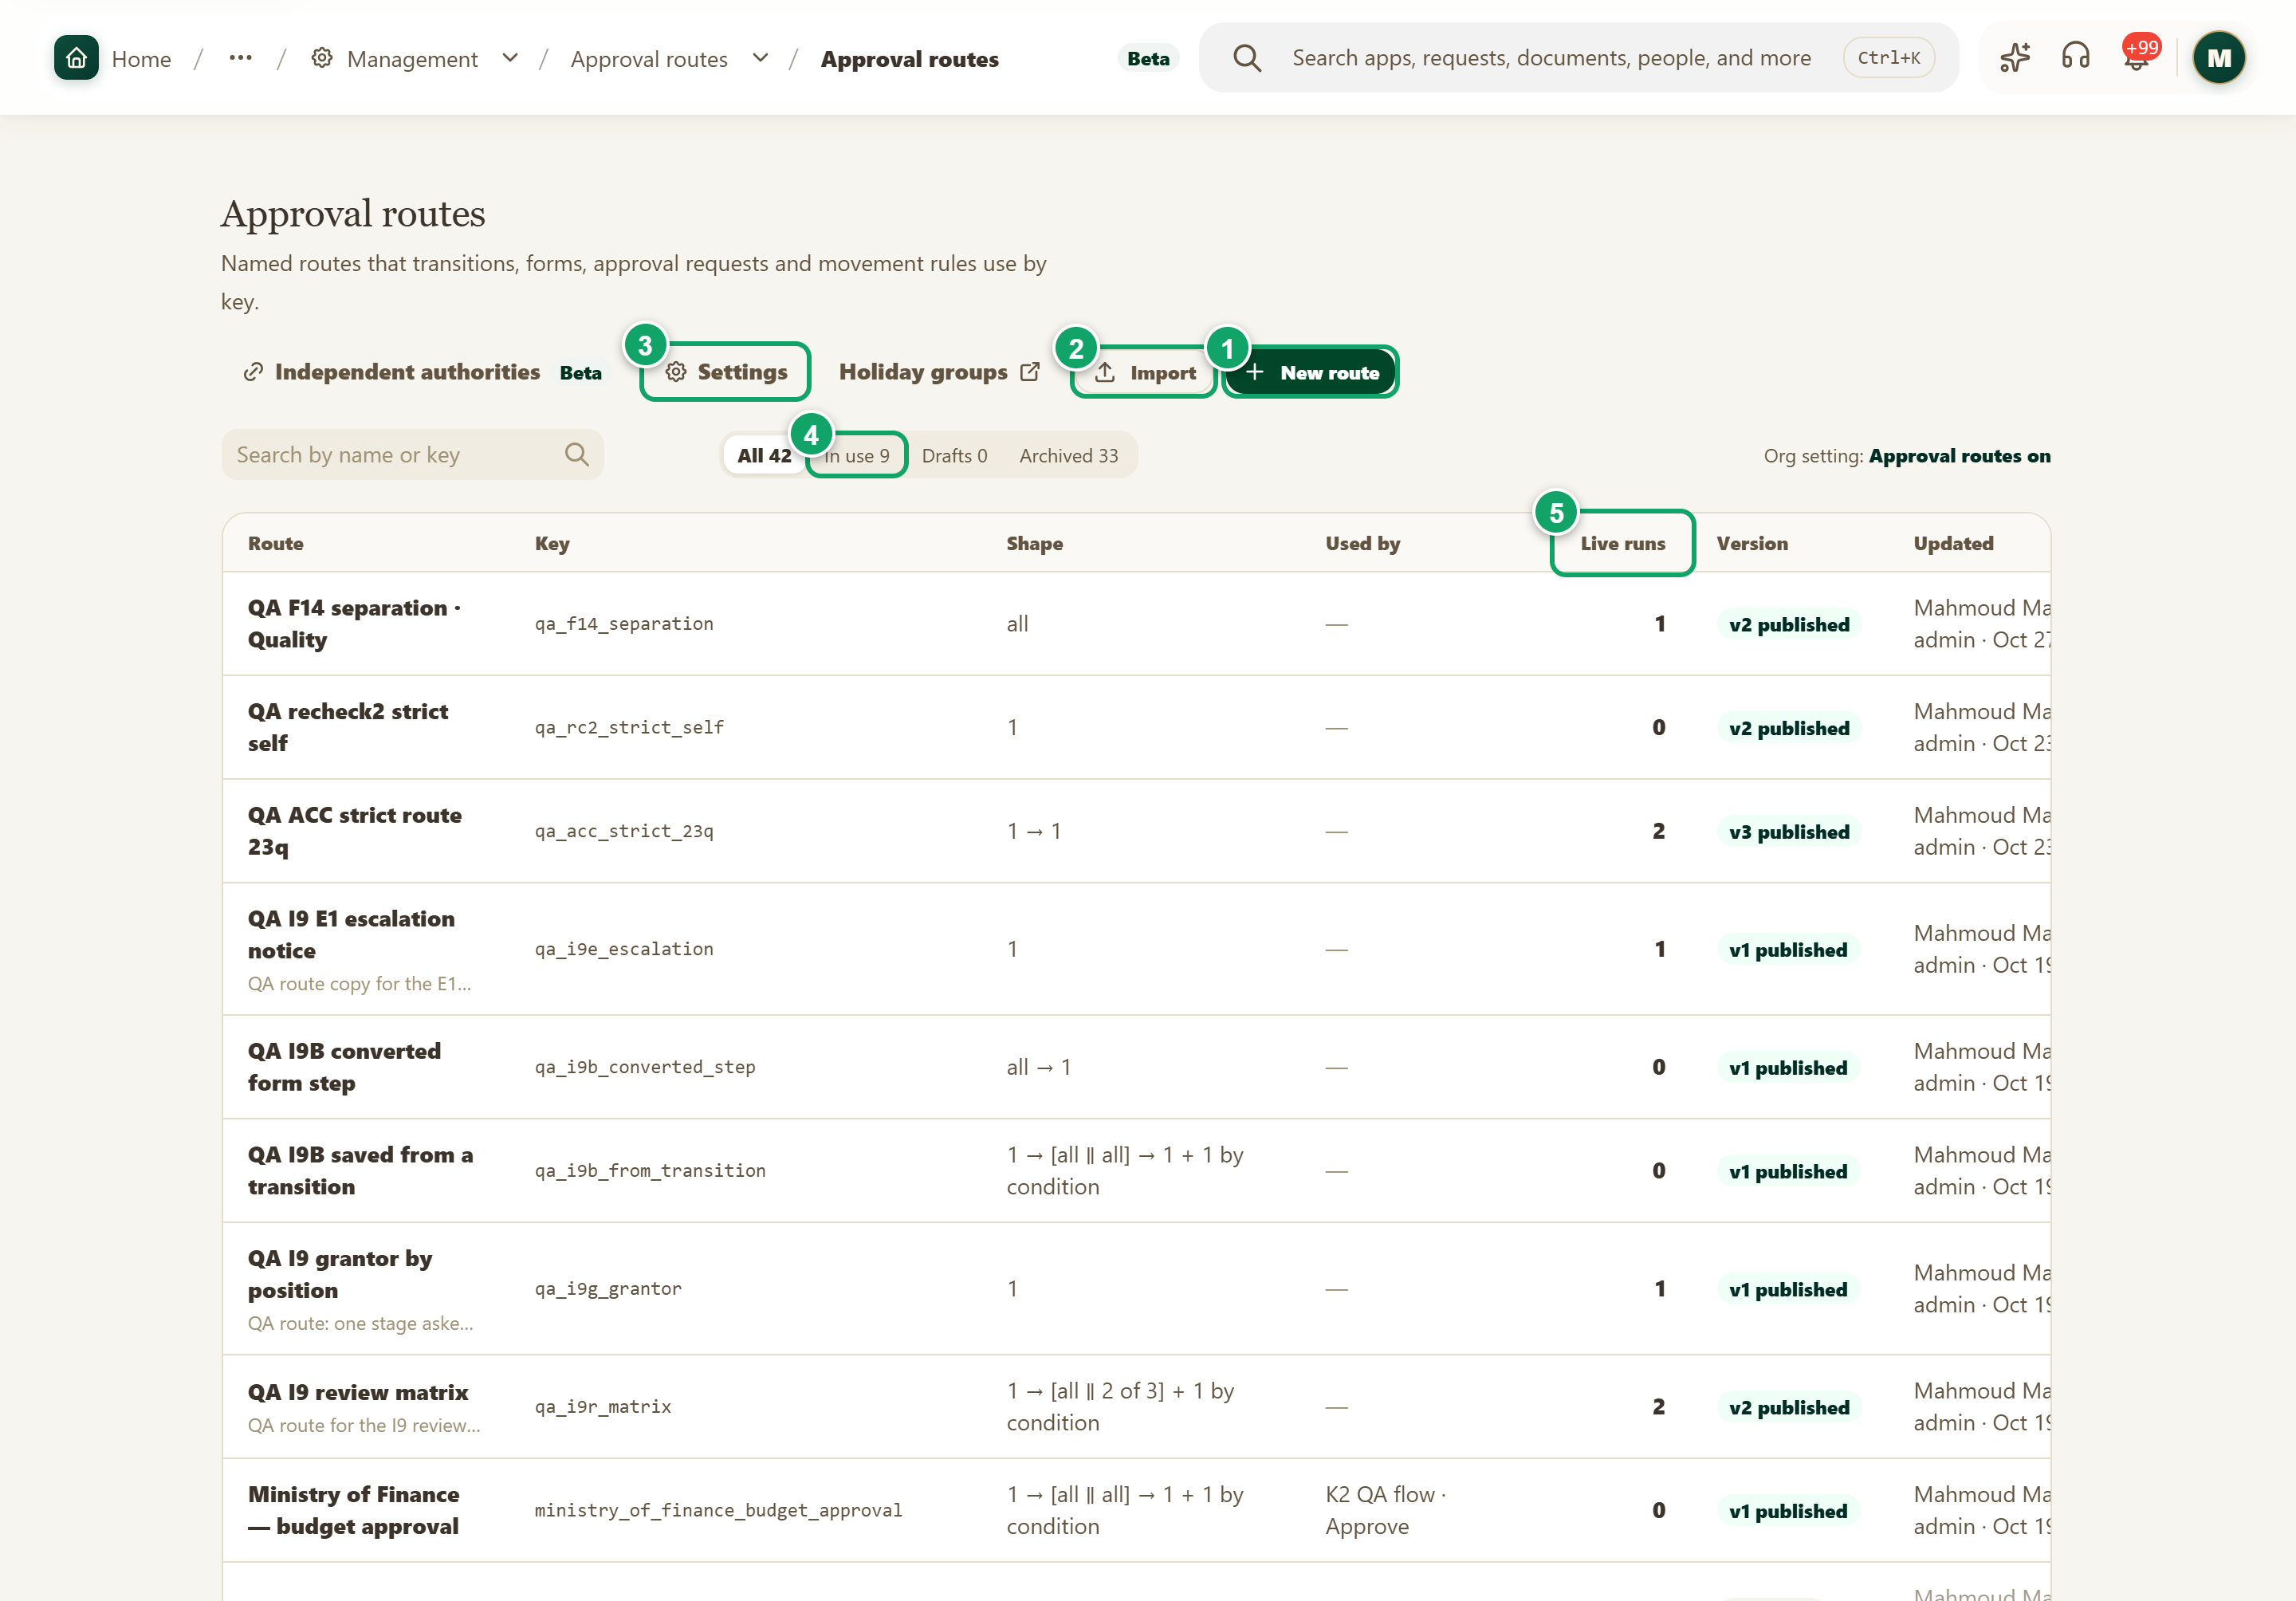
\includegraphics[width=0.95\linewidth,height=0.72\textheight,keepaspectratio]{figures/screens/ch08-approval-routes-en.png}
\caption{The approval route library}
\label{fig:settings-approval-routes-screen}
\shotnote{The library holds the organization’s routes. The “Shape” column sums up each route’s approval order, and “Used by” shows what depends on it. The routes shown are test routes. ① “New route”. ② “Import”: adds an exported route file as a draft. ③ “Settings”: the on/off switch and the working calendar. ④ “In use”: filters to routes in use. ⑤ “Live runs”: how many requests are running on the route now.}
\end{figure}

\begin{figure}[H]
\centering
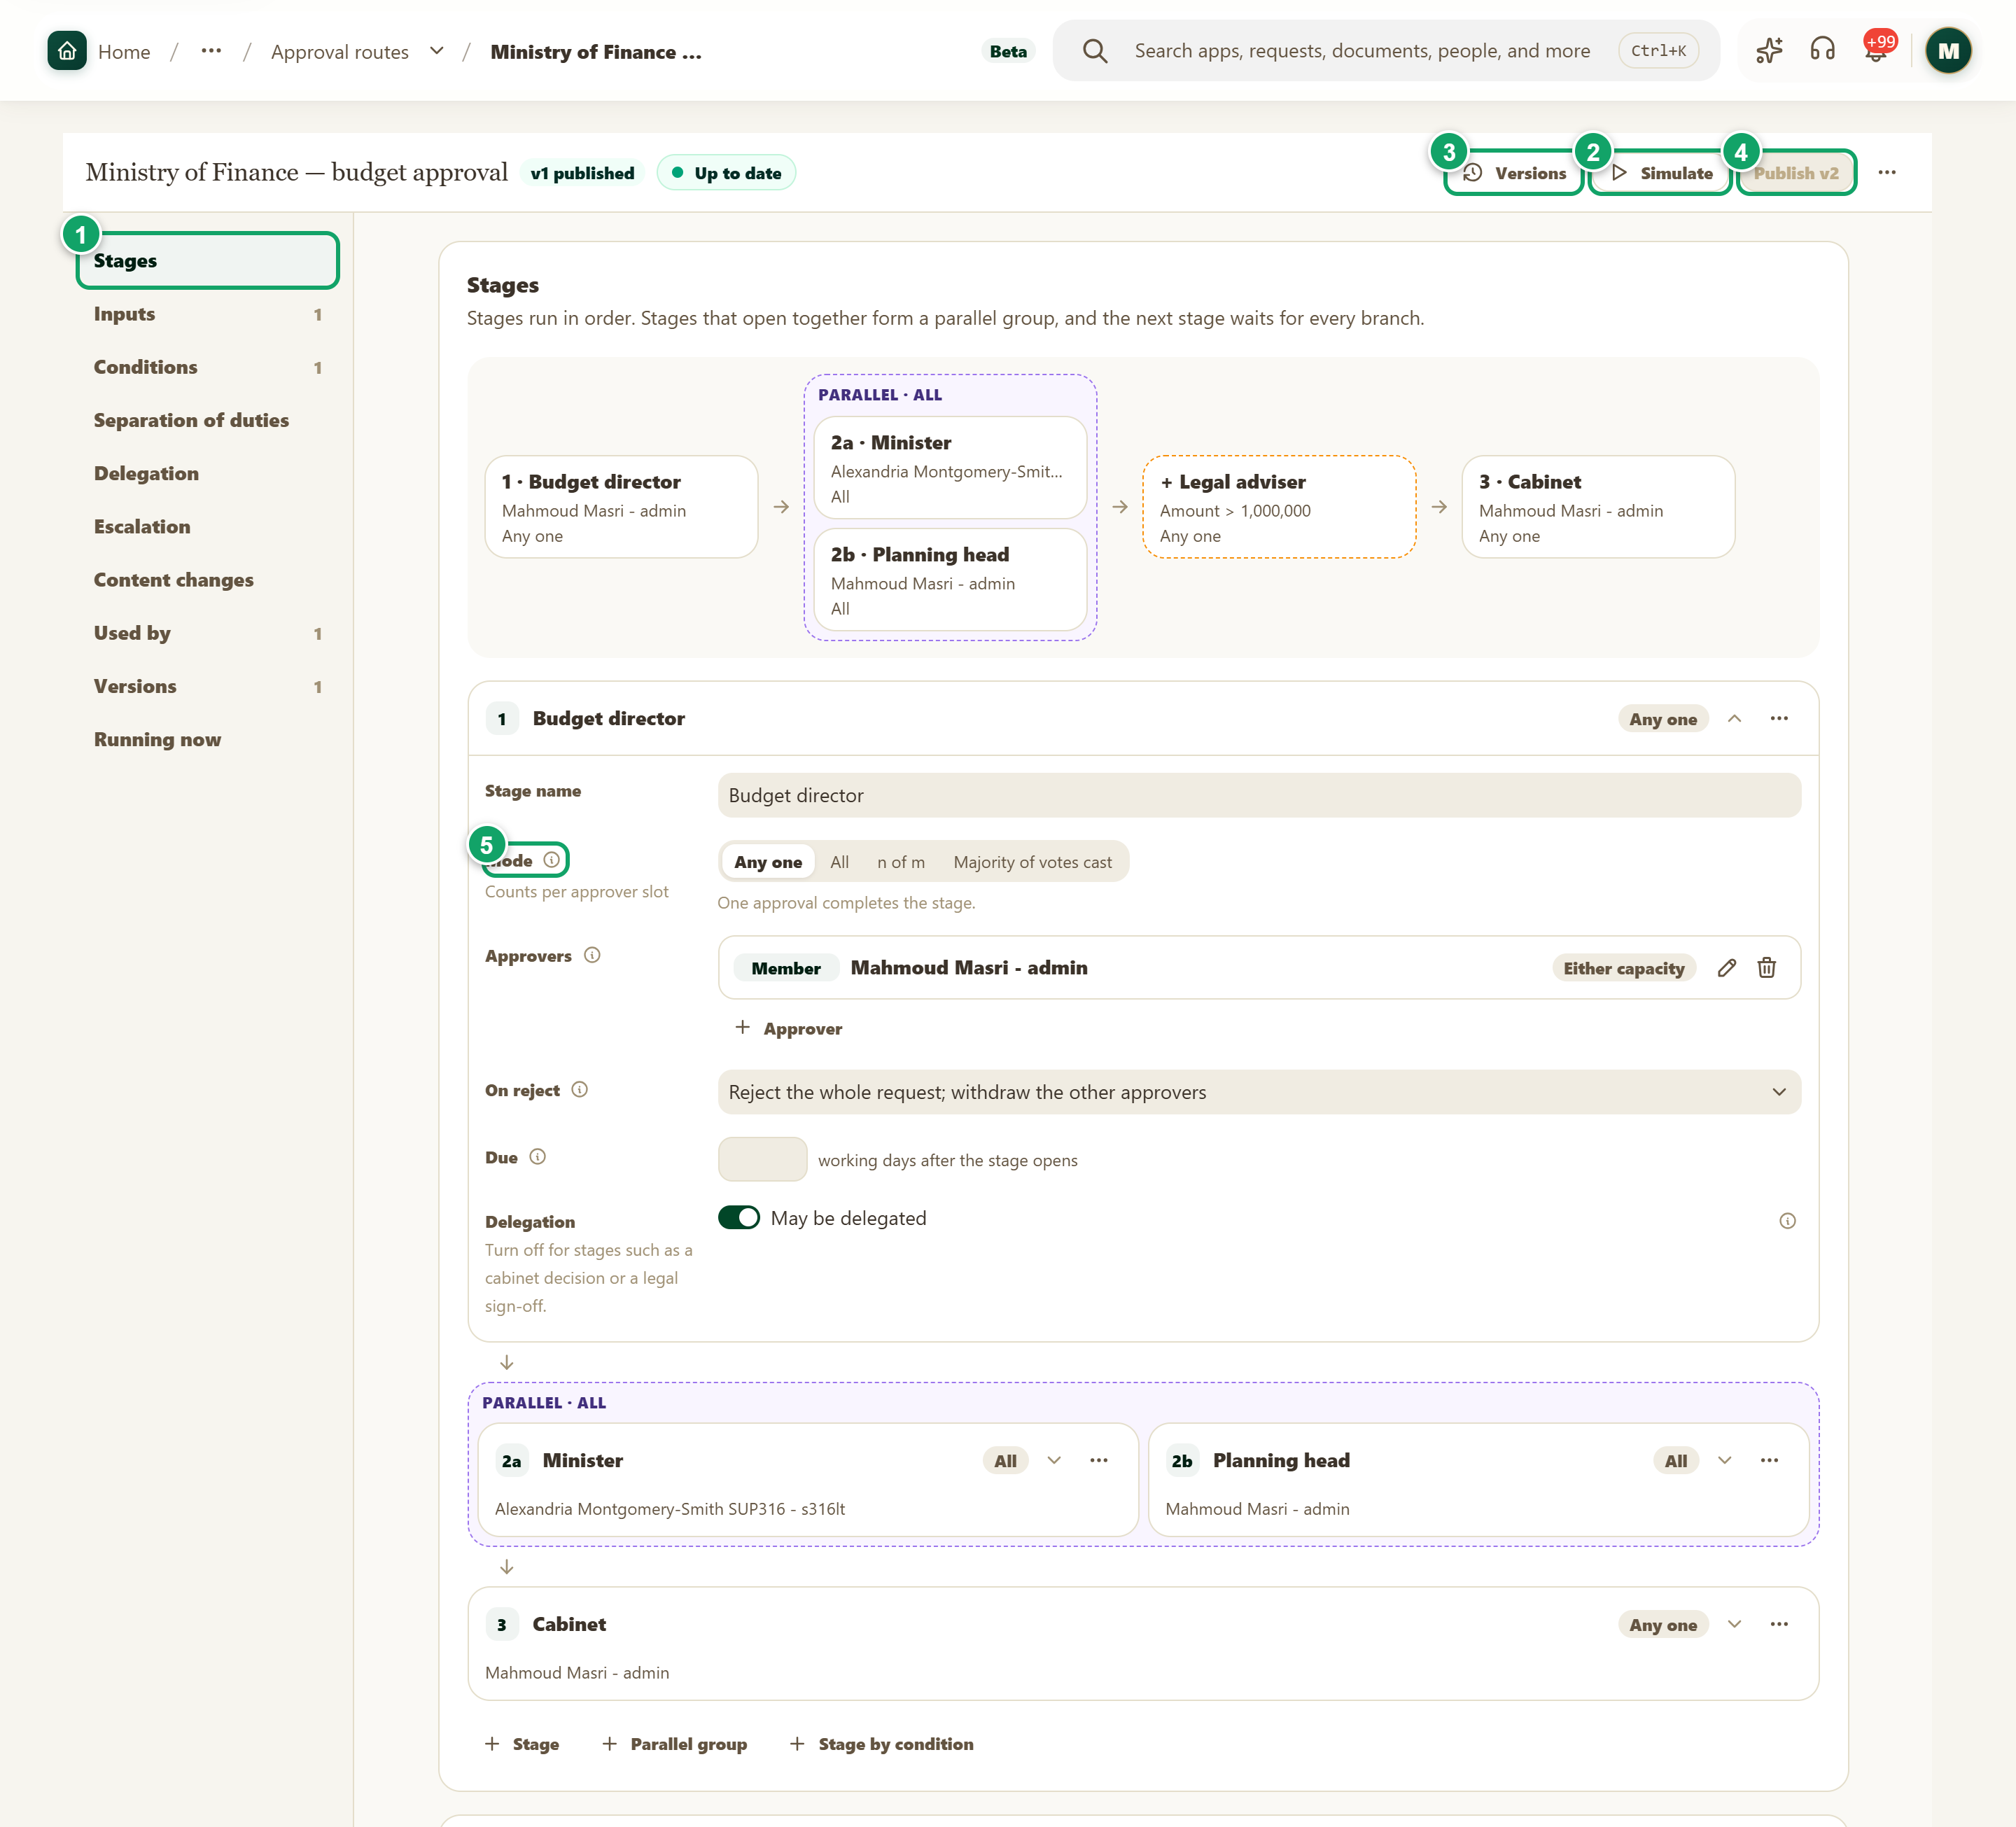
\includegraphics[width=0.95\linewidth,height=0.72\textheight,keepaspectratio]{figures/screens/ch08-approval-routes-editor-en.png}
\caption{The route editor: stages}
\label{fig:settings-approval-routes-editor-screen}
\shotnote{The editor shows the whole route shape, then the details of each stage. The next table explains the other route sections. ① “Stages”: the section list. ② “Simulate”: tries the route with sample values; nothing is saved and nobody is notified. ③ “Versions”. ④ “Publish v…”: works when the draft has changes and no errors. ⑤ “Mode”: how many approvals complete the stage.}
\end{figure}

\begin{table}[H]
\centering
\caption{What do you record in a route?}
\label{tab:settings-approval-routes-fields}
\begin{tabularx}{\linewidth}{R{4.2cm} Y}
\rcHeaderRow
\thh{Section} & \thh{What you set there}\\
“Stages” & Each stage’s name and “Mode”: “Any one”, “All”, “n of m” or “Majority of votes cast”. Then “Approvers” (member, position, role, expression or authority matrix), “On reject” and “Due”. Stages can run in parallel.\\
“Inputs” & Values each place of use maps to its own fields, such as an amount, so one route fits different record types.\\
“Conditions” & Rules that add stages when true, such as a legal adviser above a certain amount.\\
“Separation of duties” & Who may decide: stopping the requester from approving, one decision per person, requiring a signature, and allowing a send-back for changes.\\
“Delegation” & Whether a turn can be handed to someone else for a period, to whom, and whether the delegate signs.\\
“Escalation” & The day calendar, the default due time, and the steps that chase late approvers. Kayan never approves or rejects on its own.\\
“Content changes” & What happens to approvals if the record changes during the route: keep them, restart the whole route, or restart from the changed stage.\\
“Used by”, “Versions” and “Running now” & Where the route is used, its published versions, and the requests running now.\\
\end{tabularx}
\end{table}

A version is a published copy that never changes. Your edits save automatically to a draft that affects no request until you publish it, and each request records the version it started on.

\begin{figure}[H]
\centering
\begin{tikzpicture}[node distance=0.5cm]
\node[stepBox] (a) {Edits save to a draft};
\node[stepBox,below=of a] (b) {The administrator publishes the version};
\node[stepBox,below=of b] (c) {New requests start on the new version};
\node[stepBox,below=of c] (d) {Any later edit starts a new draft};
\draw[flowsTo] (a) -- (b);
\draw[flowsTo] (b) -- (c);
\draw[flowsTo] (c) -- (d);
\end{tikzpicture}
\rclegend
\caption{From a draft to a published version}
\label{fig:settings-approval-routes-versions}
\shotnote{The diagram shows why editing a route is safe: publishing is the step that makes a change take effect. Requests that started before publishing finish on their old version, so do not expect the change to reach them.}
\end{figure}

\begin{figure}[H]
\centering
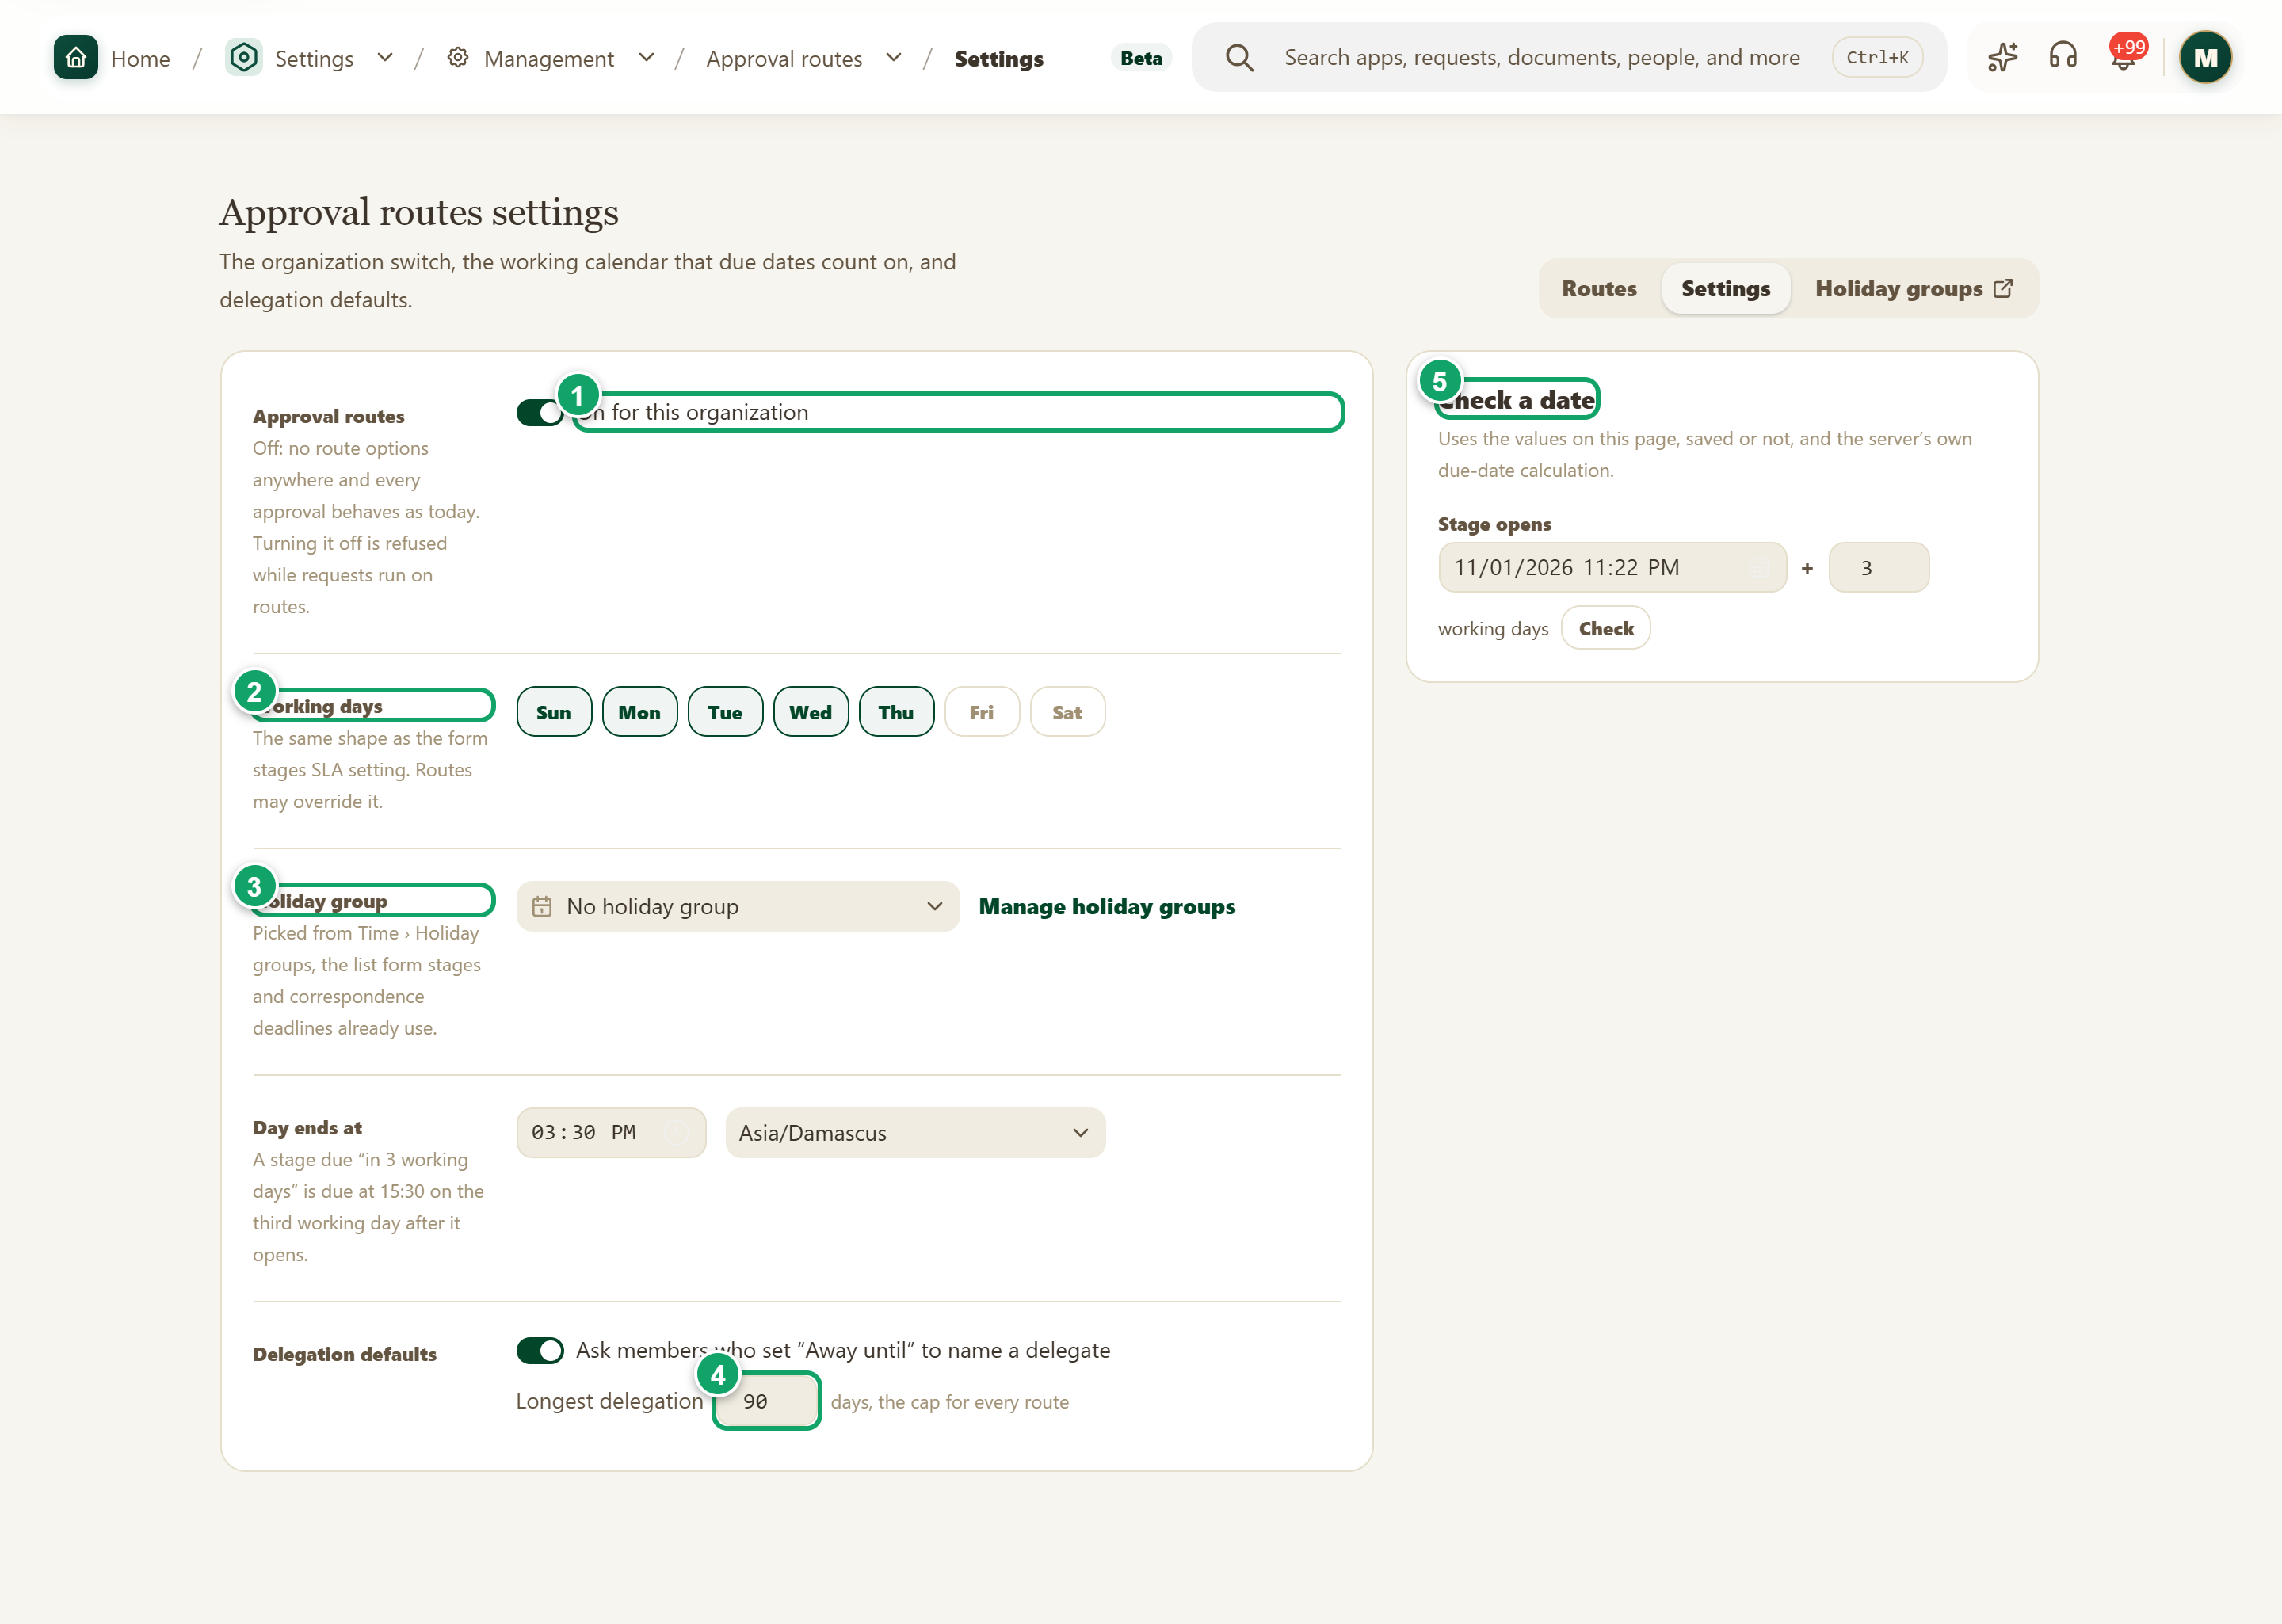
\includegraphics[width=0.95\linewidth,height=0.72\textheight,keepaspectratio]{figures/screens/ch08-approval-routes-settings-en.png}
\caption{Approval route settings}
\label{fig:settings-approval-routes-settings-screen}
\shotnote{This page holds decisions that apply to every route, chiefly the working calendar that due dates count on. You can try the calendar before saving it. ① “On for this organization”: when off, route options disappear; turning it off is refused while requests are running. ② “Working days”. ③ “Holiday group”. ④ “Longest delegation”. ⑤ “Check a date”: works out the due date from the day a stage opens.}
\end{figure}

\begin{enumerate}
\item Open “Settings”, then “Approval routes”, and confirm that “Approval routes on” is shown.
\item Press “New route”, enter the title and key, then press “Create route”. The key cannot change afterwards.
\item Add the stages, set “Mode” and “Approvers” for each, and review the other sections.
\item Press “Simulate” to try the route, then fix any problems: errors block publishing, warnings do not.
\item Press “Publish v…” and confirm, then pick the route from the transition, form or request that needs it.
\end{enumerate}

\textbf{Check:} The route shows its published version chip, and its place of use appears under “Used by”. A route that is used or published cannot be deleted; when you no longer need it, move its users to another route and press “Archive”. “Delete draft” applies only to a route never published.

\section{Evaluation templates}
\label{sec:settings-feature-evaluation-templates}

An evaluation template is a reusable scorecard: criteria, a scoring model, and optional bands that turn a total into a recommended outcome. Record types pick a template for each kind of evaluation, such as a supplier review or an interview, so everyone scores against the same criteria. Anyone who can edit entities or manage templates can read the library; editing and publishing each have their own permission.

\begin{rcnote}[Example: Horizon]
The system administrator presses “New template” at ① to create a “Hospitality supplier review” template from a starter in “Procurement pack” at ②. The administrator then adds a mandatory check for a commercial register and publishes the version, so Omar Haddad can use it when reviewing suppliers.
\end{rcnote}

\begin{figure}[H]
\centering
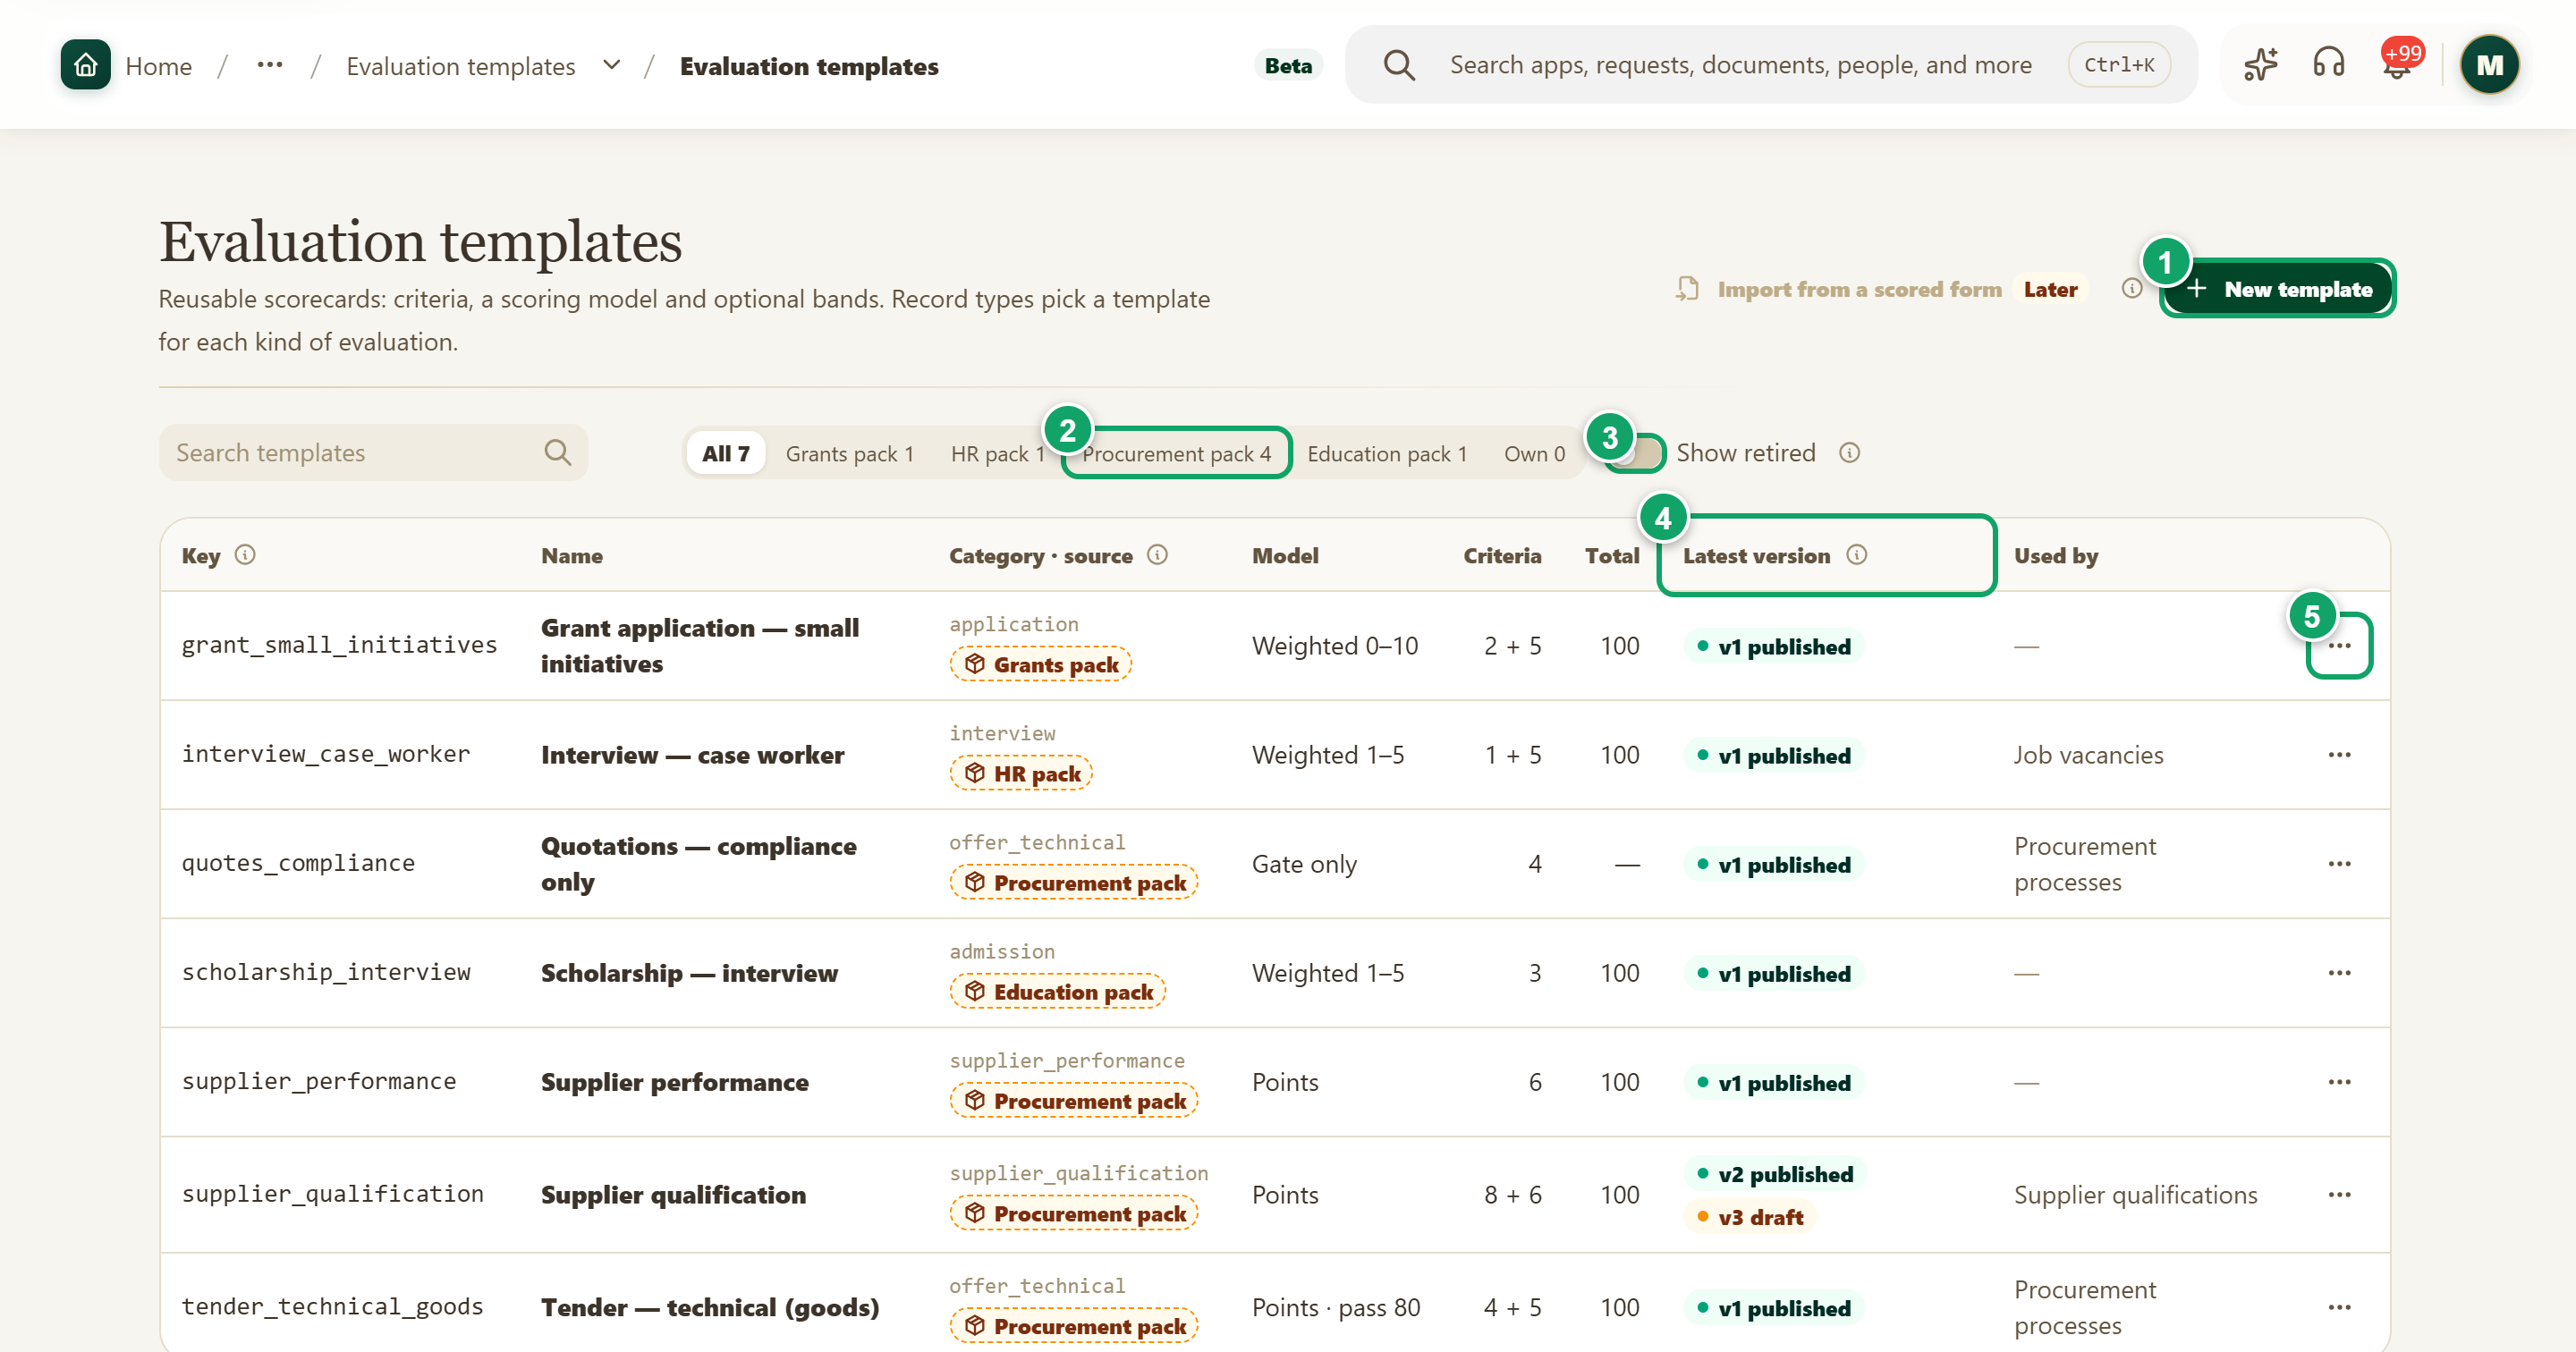
\includegraphics[width=0.95\linewidth,height=0.72\textheight,keepaspectratio]{figures/screens/ch08-evaluation-templates-en.png}
\caption{The evaluation template library}
\label{fig:settings-evaluation-templates-screen}
\shotnote{The library shows templates with their scoring model, number of criteria and latest version. These are starter templates installed in the test organization, and “Import from a scored form” is marked “Later” and is not available. ① “New template”. ② Filters by the template’s source. ③ “Show retired”. ④ “Latest version”. ⑤ The template menu: copy it, see its versions, or “Retire”.}
\end{figure}

\begin{figure}[H]
\centering
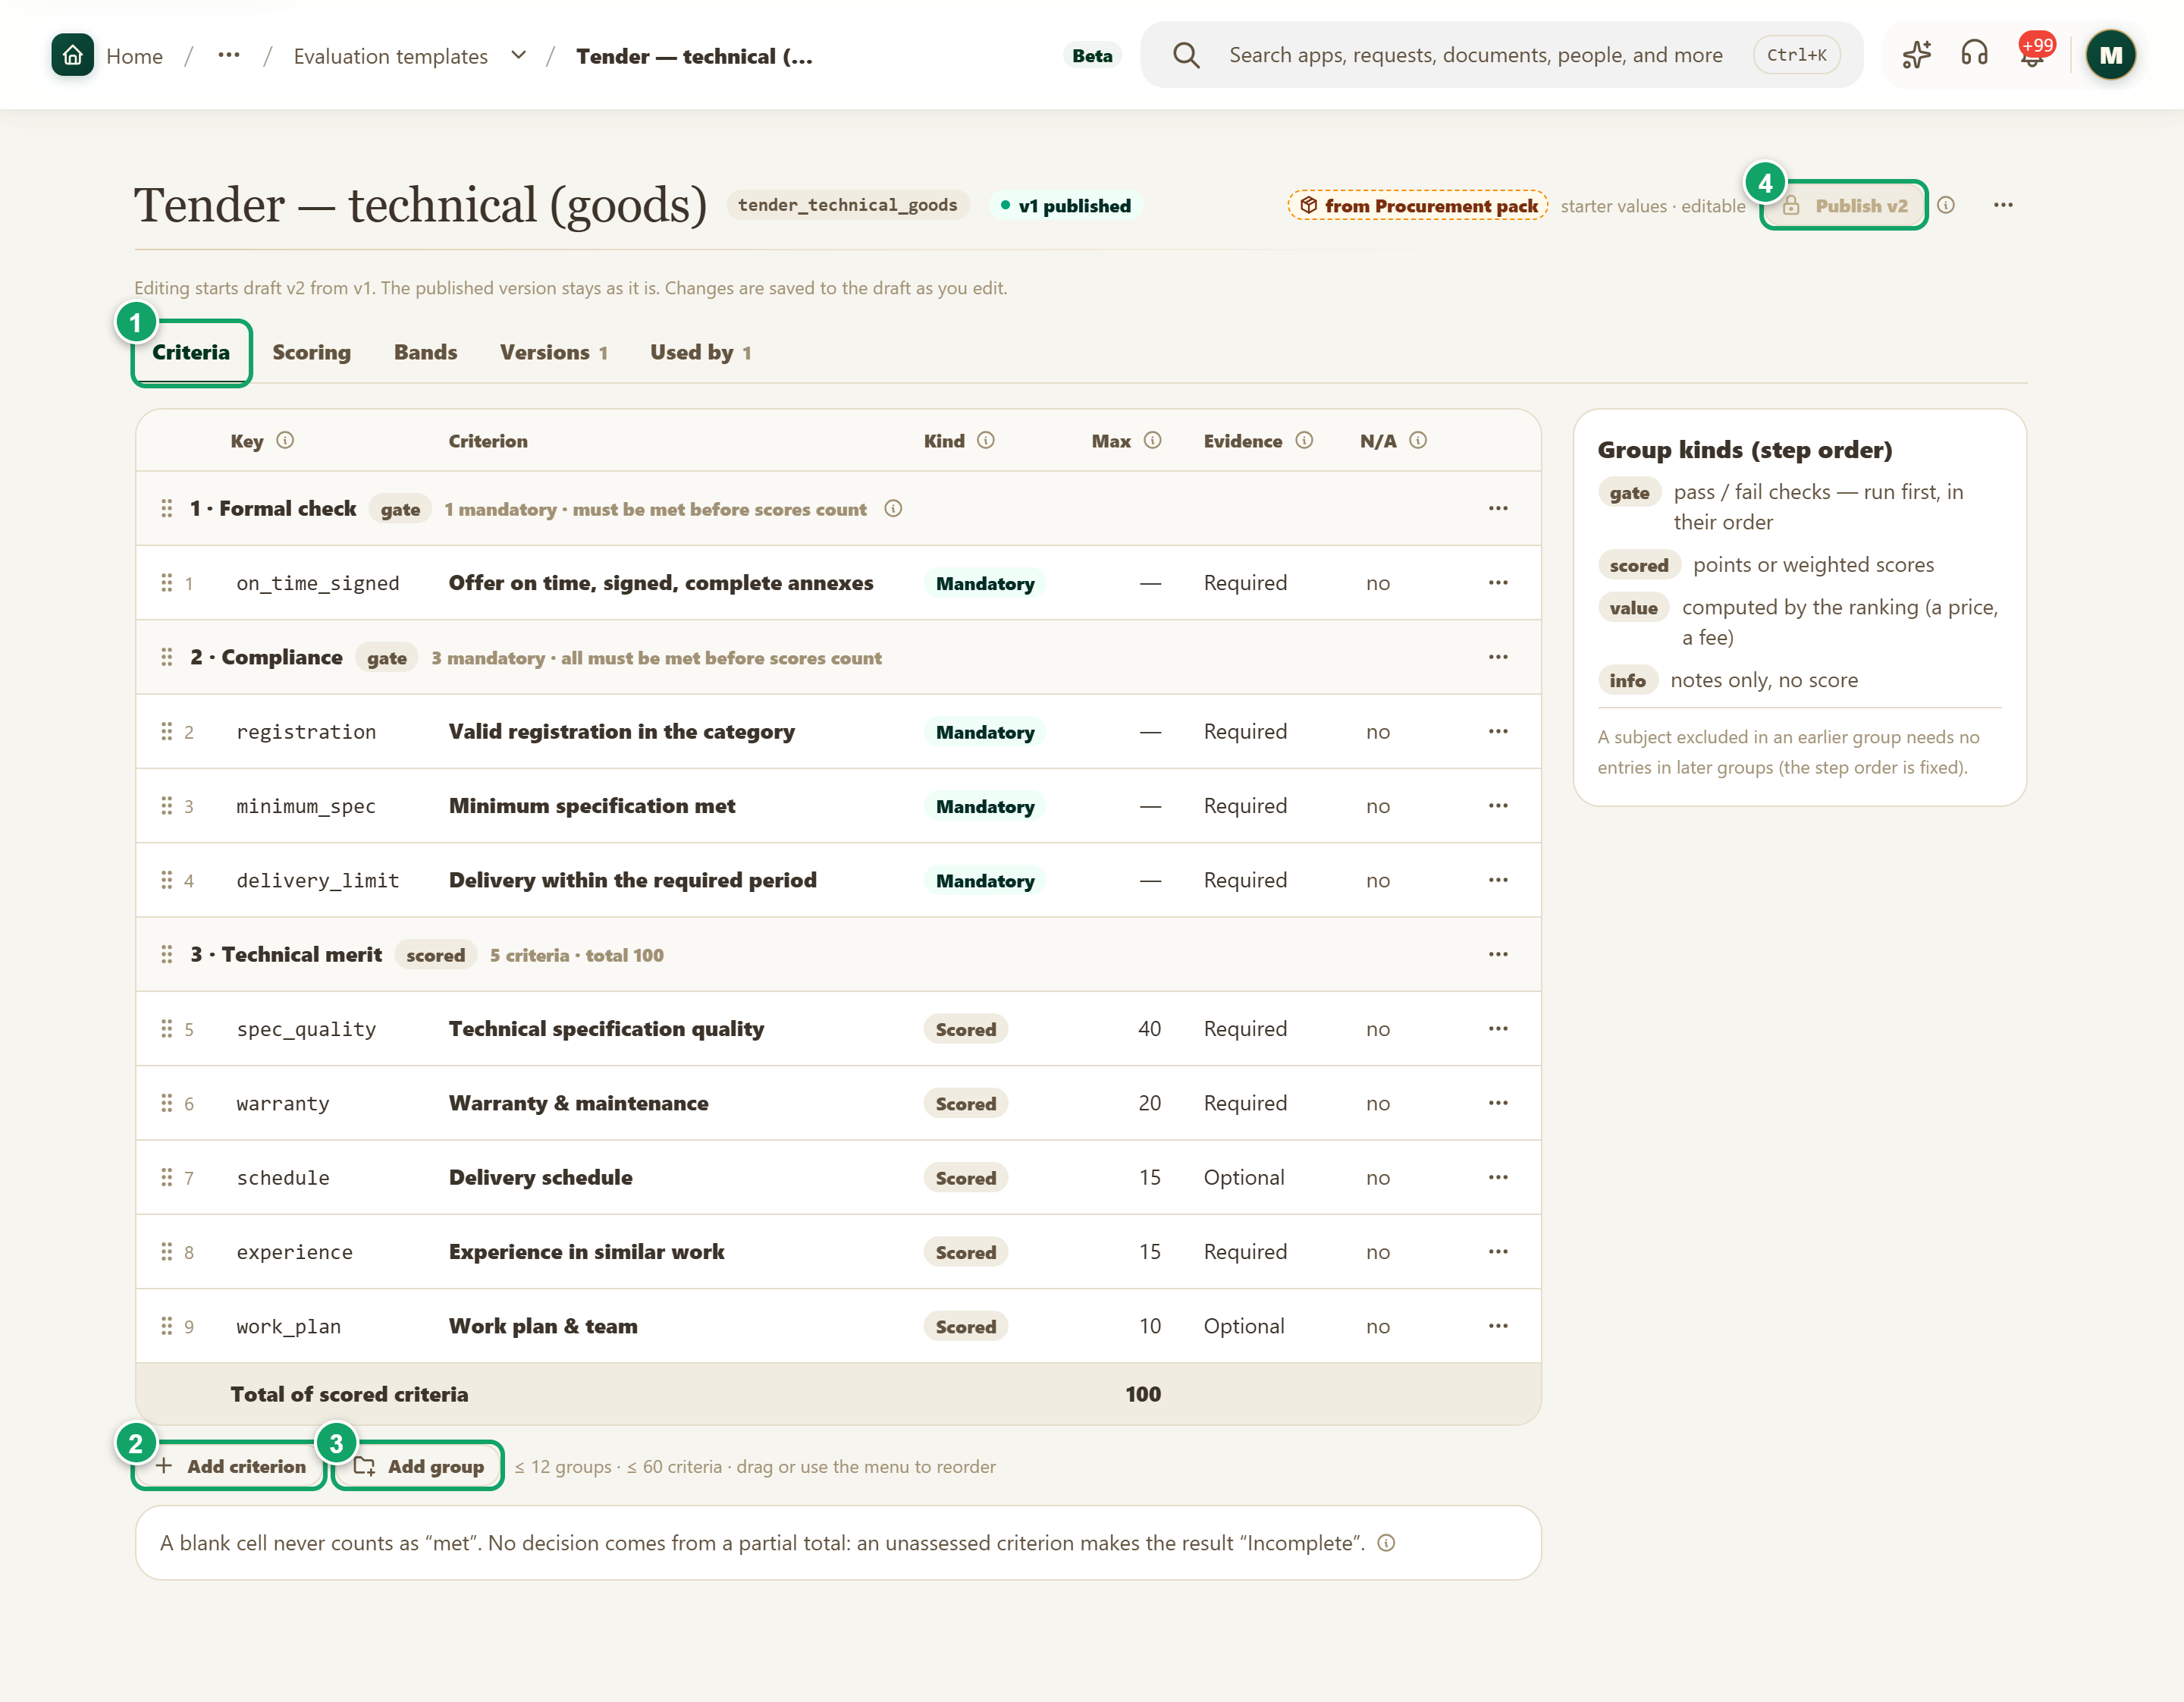
\includegraphics[width=0.95\linewidth,height=0.72\textheight,keepaspectratio]{figures/screens/ch08-evaluation-templates-criteria-en.png}
\caption{The Criteria tab}
\label{fig:settings-evaluation-templates-criteria-screen}
\shotnote{Criteria sit in groups that run in order, so a subject excluded in a “gate” group needs no entries in later groups. Any edit here starts a draft, and the published version stays as it is. ① “Criteria”. ② “Add criterion”. ③ “Add group”. ④ “Publish v…”: stays disabled while there is no draft.}
\end{figure}

\begin{figure}[H]
\centering
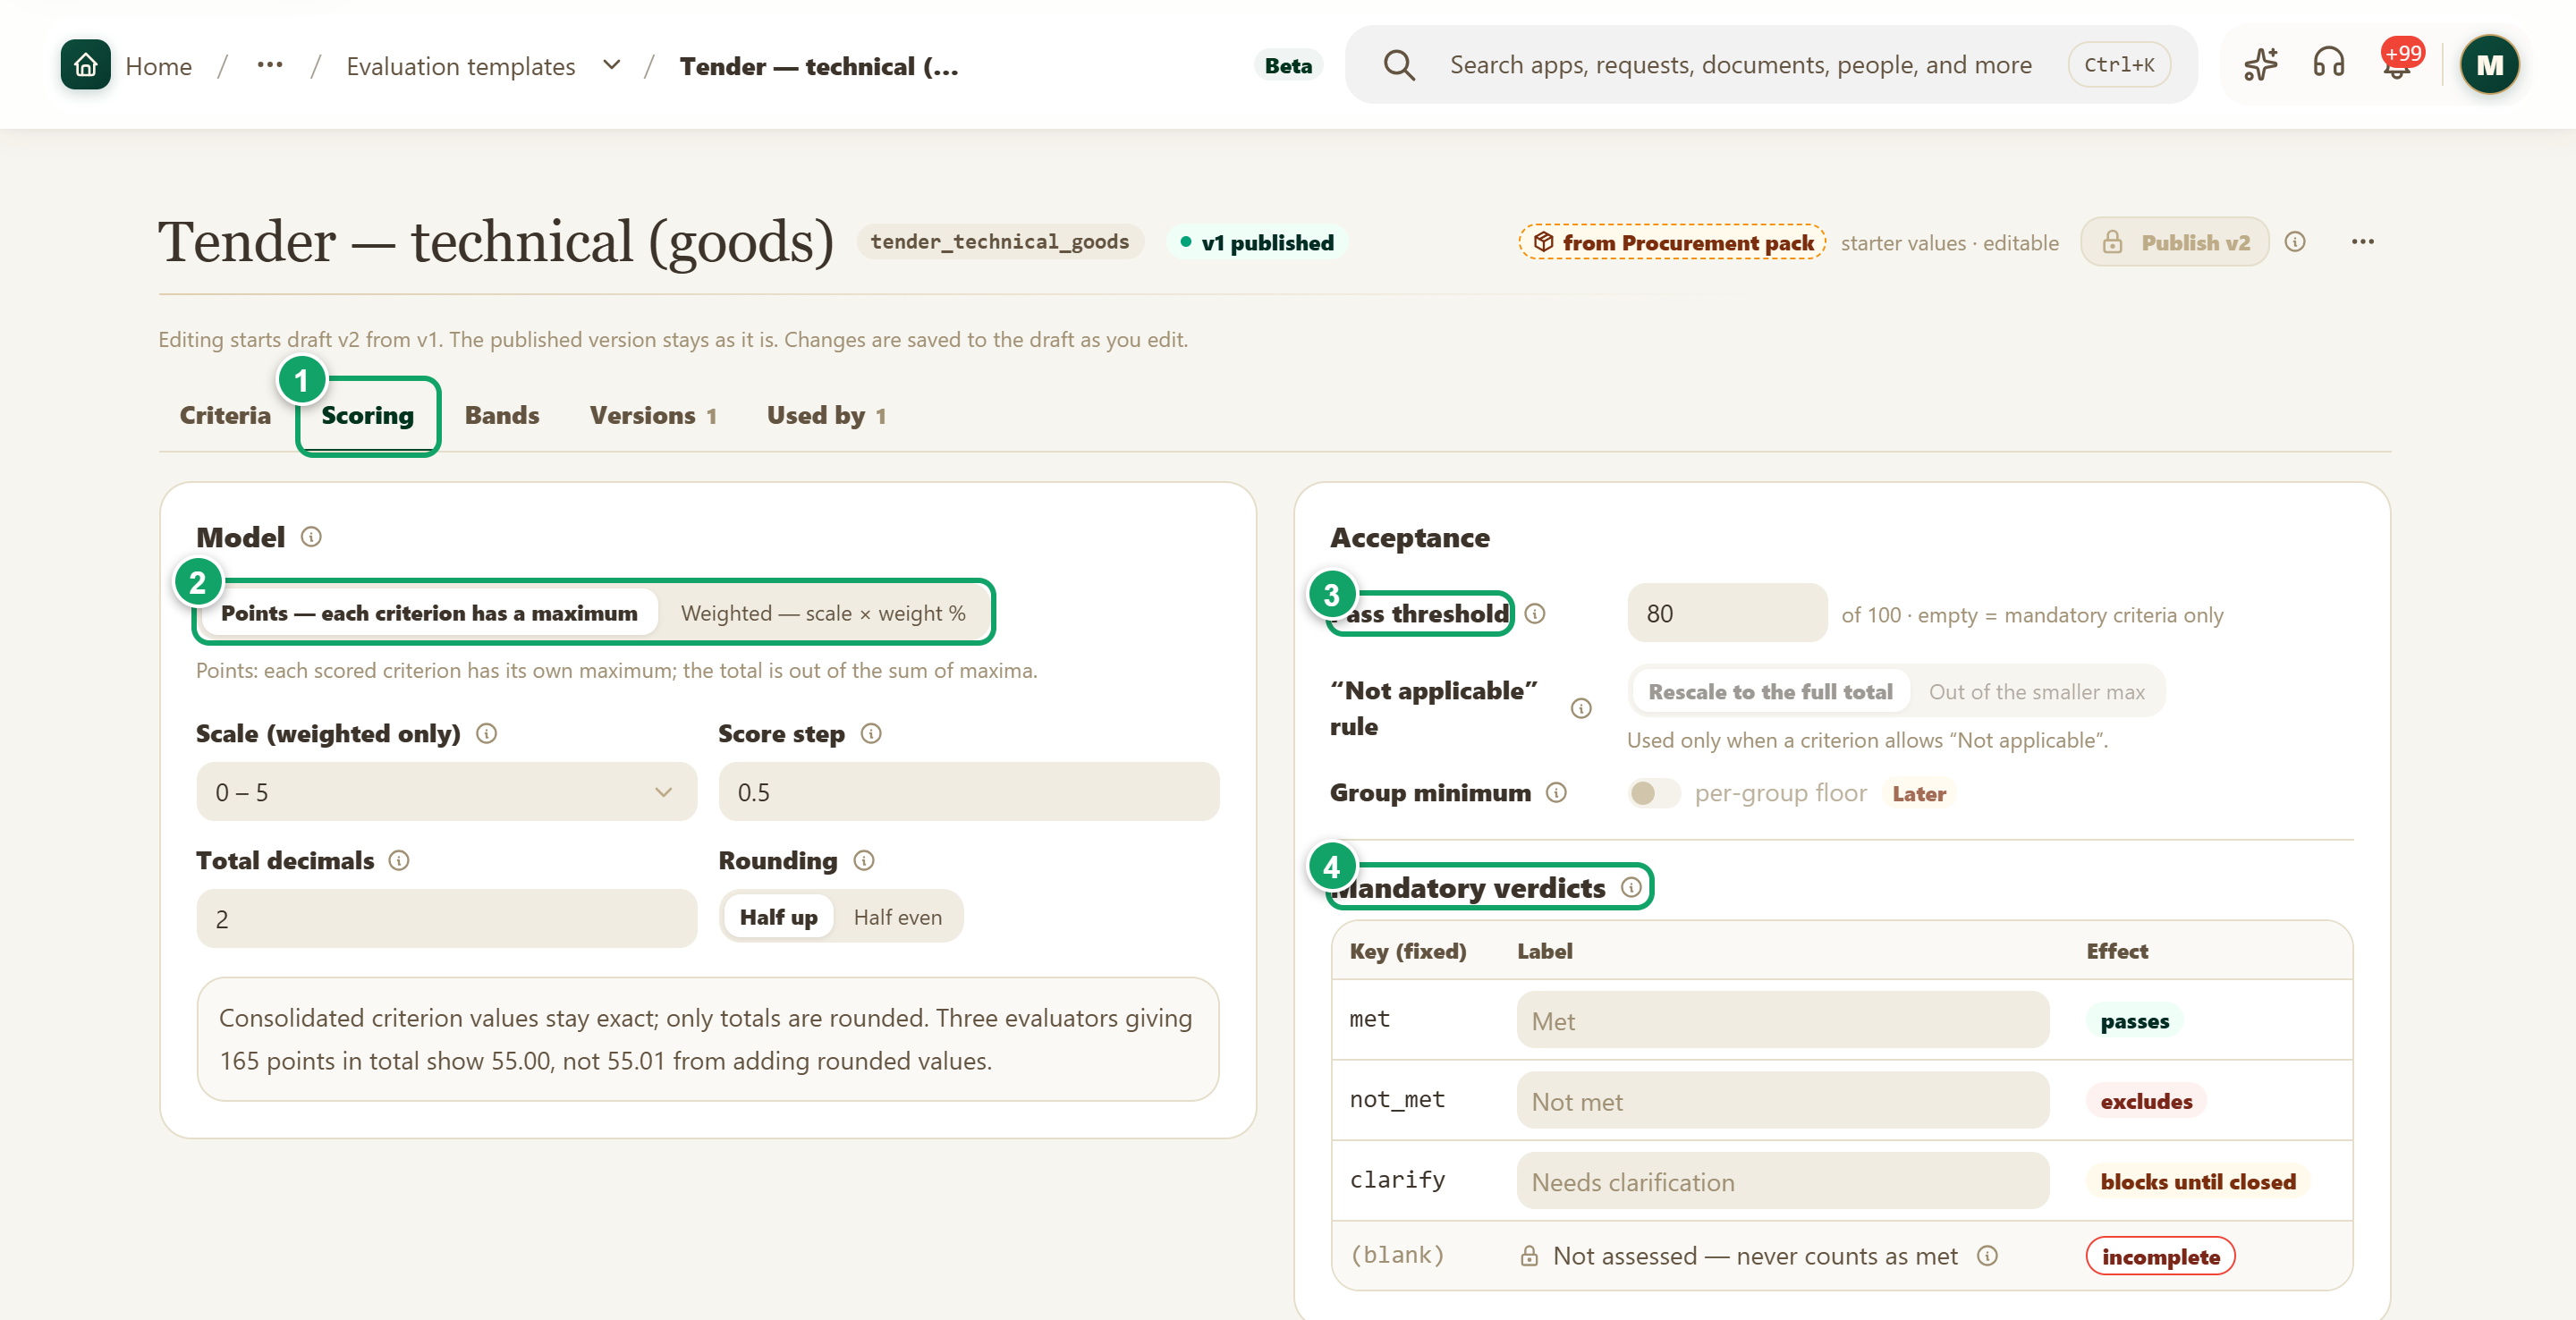
\includegraphics[width=0.95\linewidth,height=0.72\textheight,keepaspectratio]{figures/screens/ch08-evaluation-templates-scoring-en.png}
\caption{The Scoring tab}
\label{fig:settings-evaluation-templates-scoring-screen}
\shotnote{This tab sets how the total is worked out and what it takes to pass. Criterion values stay exact and only totals are rounded, so no gap comes from adding rounded values. ① “Scoring”. ② “Scoring model”: points per criterion, or a scale with weights. ③ “Pass threshold”: empty means mandatory criteria only. ④ “Mandatory verdicts”: a blank cell never counts as met.}
\end{figure}

\begin{figure}[H]
\centering
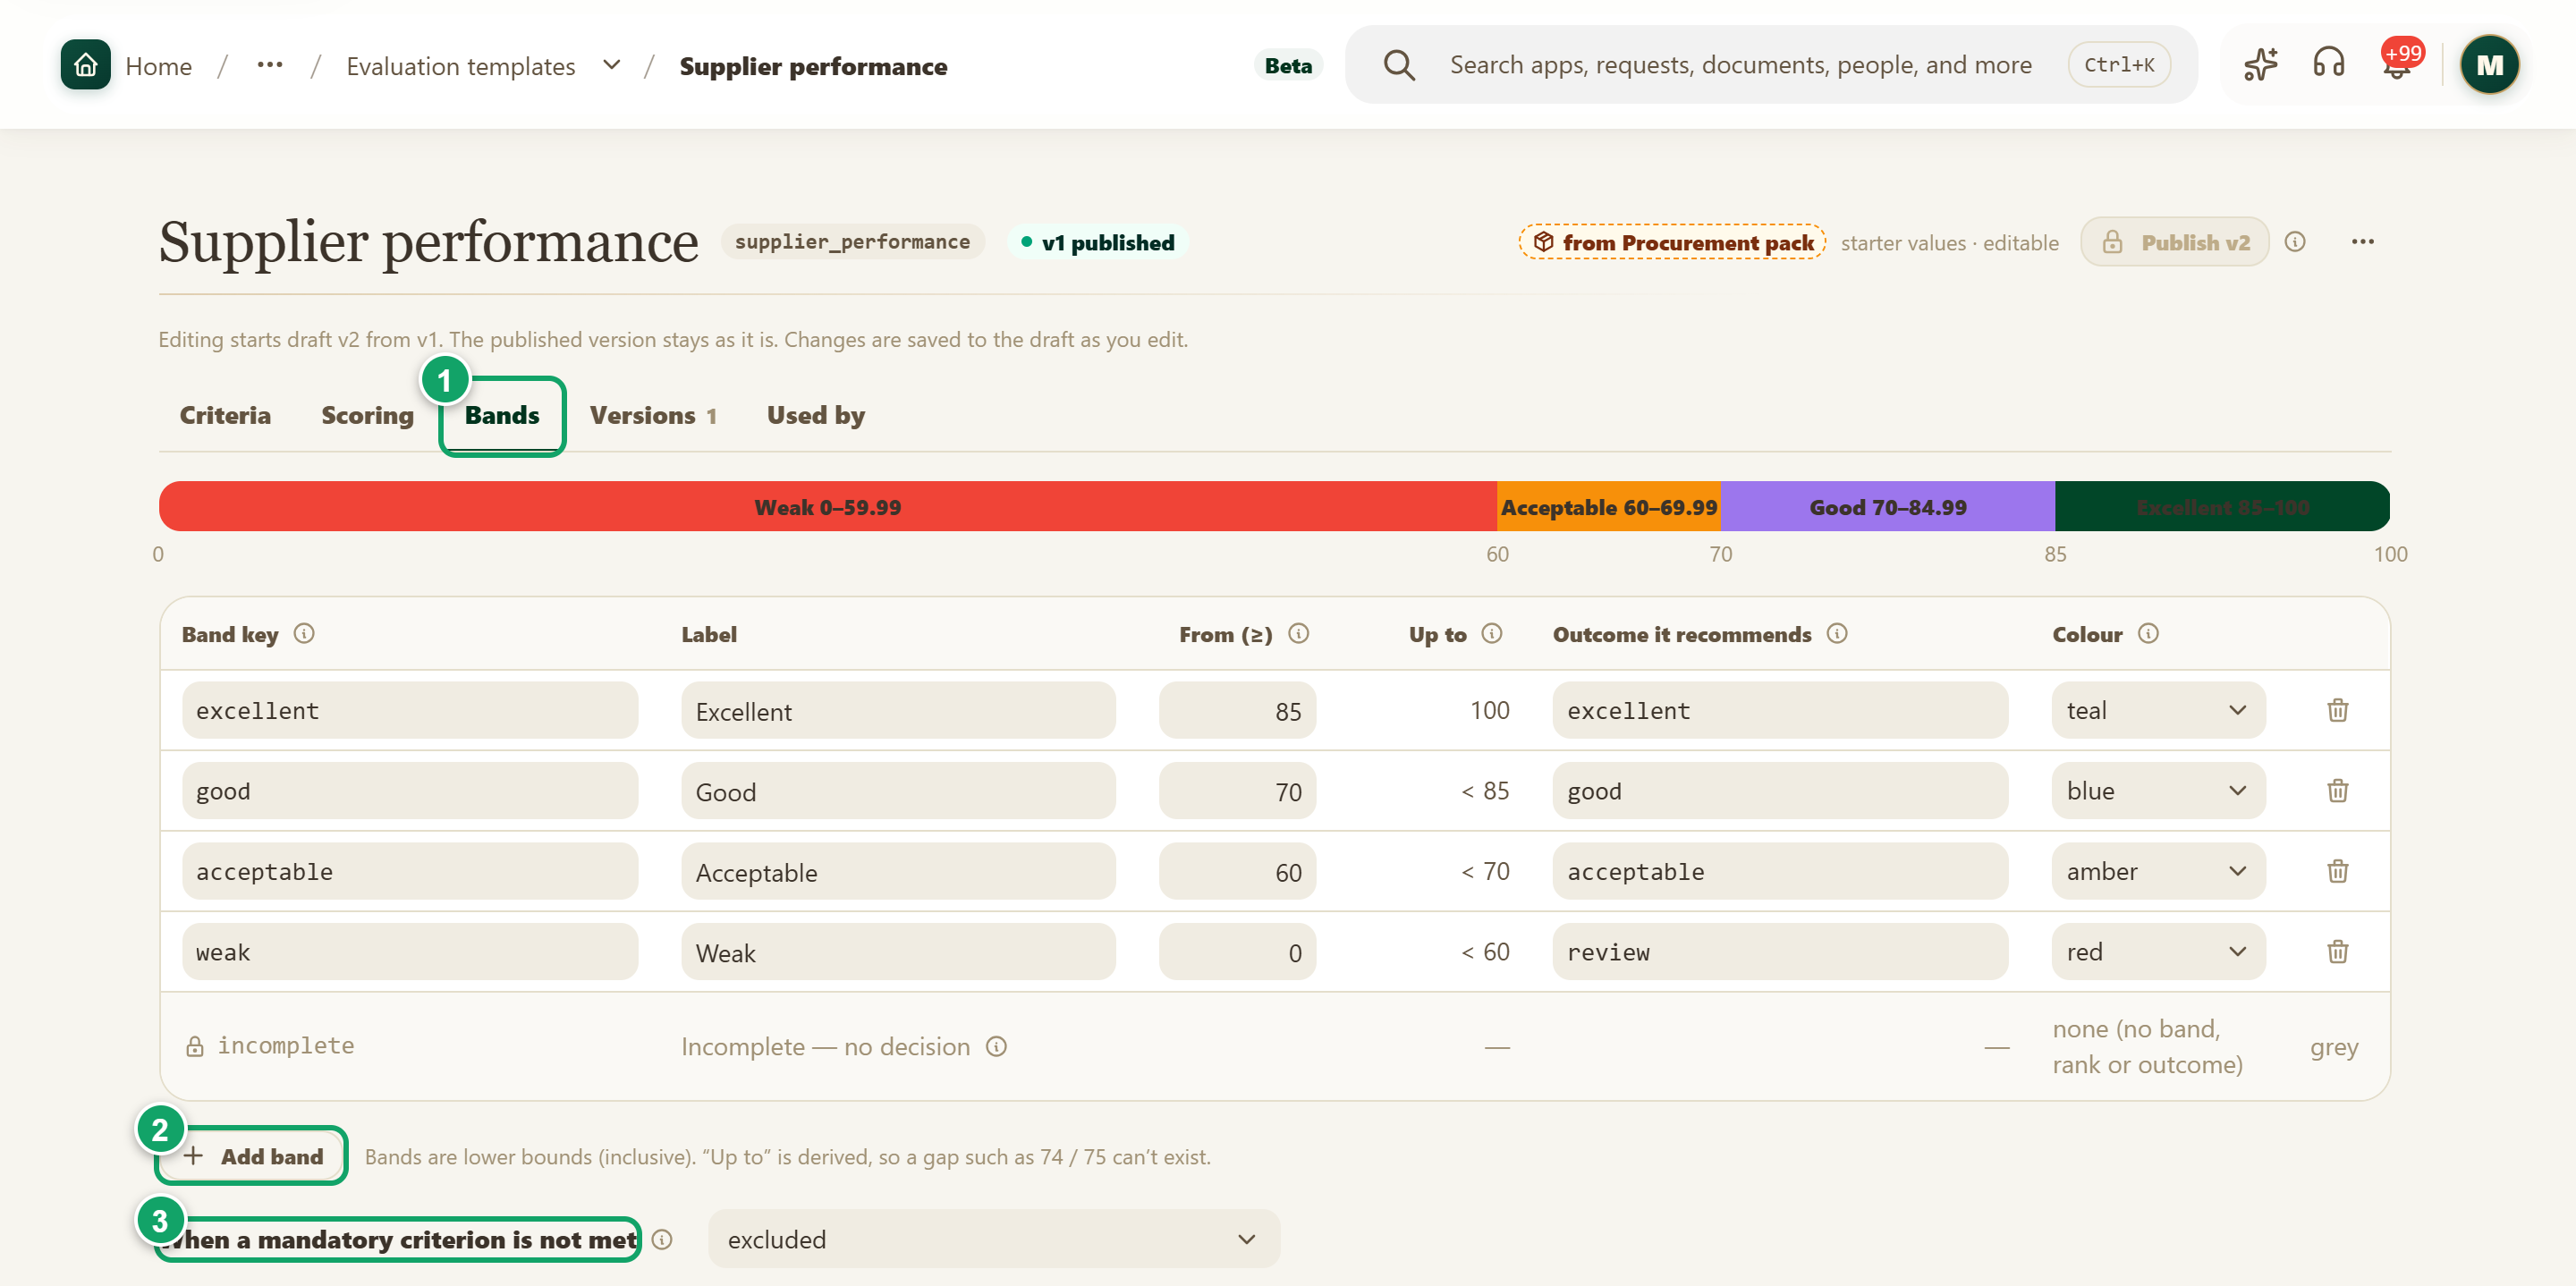
\includegraphics[width=0.95\linewidth,height=0.72\textheight,keepaspectratio]{figures/screens/ch08-evaluation-templates-bands-en.png}
\caption{The Bands tab}
\label{fig:settings-evaluation-templates-bands-screen}
\shotnote{Bands turn a total into an outcome people understand, such as acceptable or weak. Each band sets only its lower bound, so the upper bound is worked out and no gap can appear between two bands. ① “Bands”. ② “Add band”. ③ The outcome when a mandatory criterion is not met.}
\end{figure}

\begin{table}[H]
\centering
\caption{What do you record in a template?}
\label{tab:settings-evaluation-templates-fields}
\begin{tabularx}{\linewidth}{R{4.2cm} Y}
\rcHeaderRow
\thh{Part} & \thh{What you record there}\\
New template & “Key”, “Name”, “Category”, and “Start from”: blank, a starter from a pack, or a copy of another template.\\
“Criteria” & Groups of four kinds: “gate”, “scored”, “value” and “info”. Each criterion has its key, label, kind, maximum or weight, “Evidence”, guidance, and a “Not applicable” option.\\
“Scoring” & “Scoring model”, scale, “Score step”, “Total decimals”, “Rounding”, “Pass threshold” and “Mandatory verdicts”.\\
“Bands” & The band key, label, lower bound, recommended outcome and color.\\
“Versions” & Published versions with their date, publisher, note and fingerprint.\\
“Used by” & The record types using the template and their open evaluations. A record type picks the template in the Builder.\\
\end{tabularx}
\end{table}

\begin{enumerate}
\item Open “Settings”, then “Evaluation templates”, and press “New template”.
\item Enter “Key” and “Name”, choose where to begin in “Start from”, then press “Create draft”.
\item Add groups and criteria, then set “Scoring” and “Bands”. Changes save to the draft as you edit.
\item Fix the problems shown, then press “Publish v…” and write a note saying why.
\item When you no longer need a template, open its menu and press “Retire”; templates have no delete.
\end{enumerate}

\textbf{Check:} The template shows its published version chip in the library, and a record type can pick it. When you publish a new version, open evaluations stay on their pinned version and the new one applies to new evaluations only. If the publish button stays disabled, review the problems shown; weights, for example, must add up to 100.

\section{Follow-up}
\label{sec:settings-feature-followup}

This page sets the shared words that follow-up boards use to explain delay. A “stuck reason” says why a record is waiting in its stage, a “blocker type” links a record to another that keeps it from moving on, and an “intervention” is a decision asked of a higher authority to end the delay. Boards work without reasons too, but overdue rows then read “Unexplained”. Those with access can read the page; changing it needs the “Configure follow-up” permission.

\begin{rcnote}[Example: Horizon]
The system administrator presses “New reason” at ② and adds “Waiting for supplier approval”. When the Aleppo branch visit runs late, Sarah Al-Khatib picks that reason, so the board shows the time under this reason instead of as an unexplained delay.
\end{rcnote}

\begin{figure}[H]
\centering
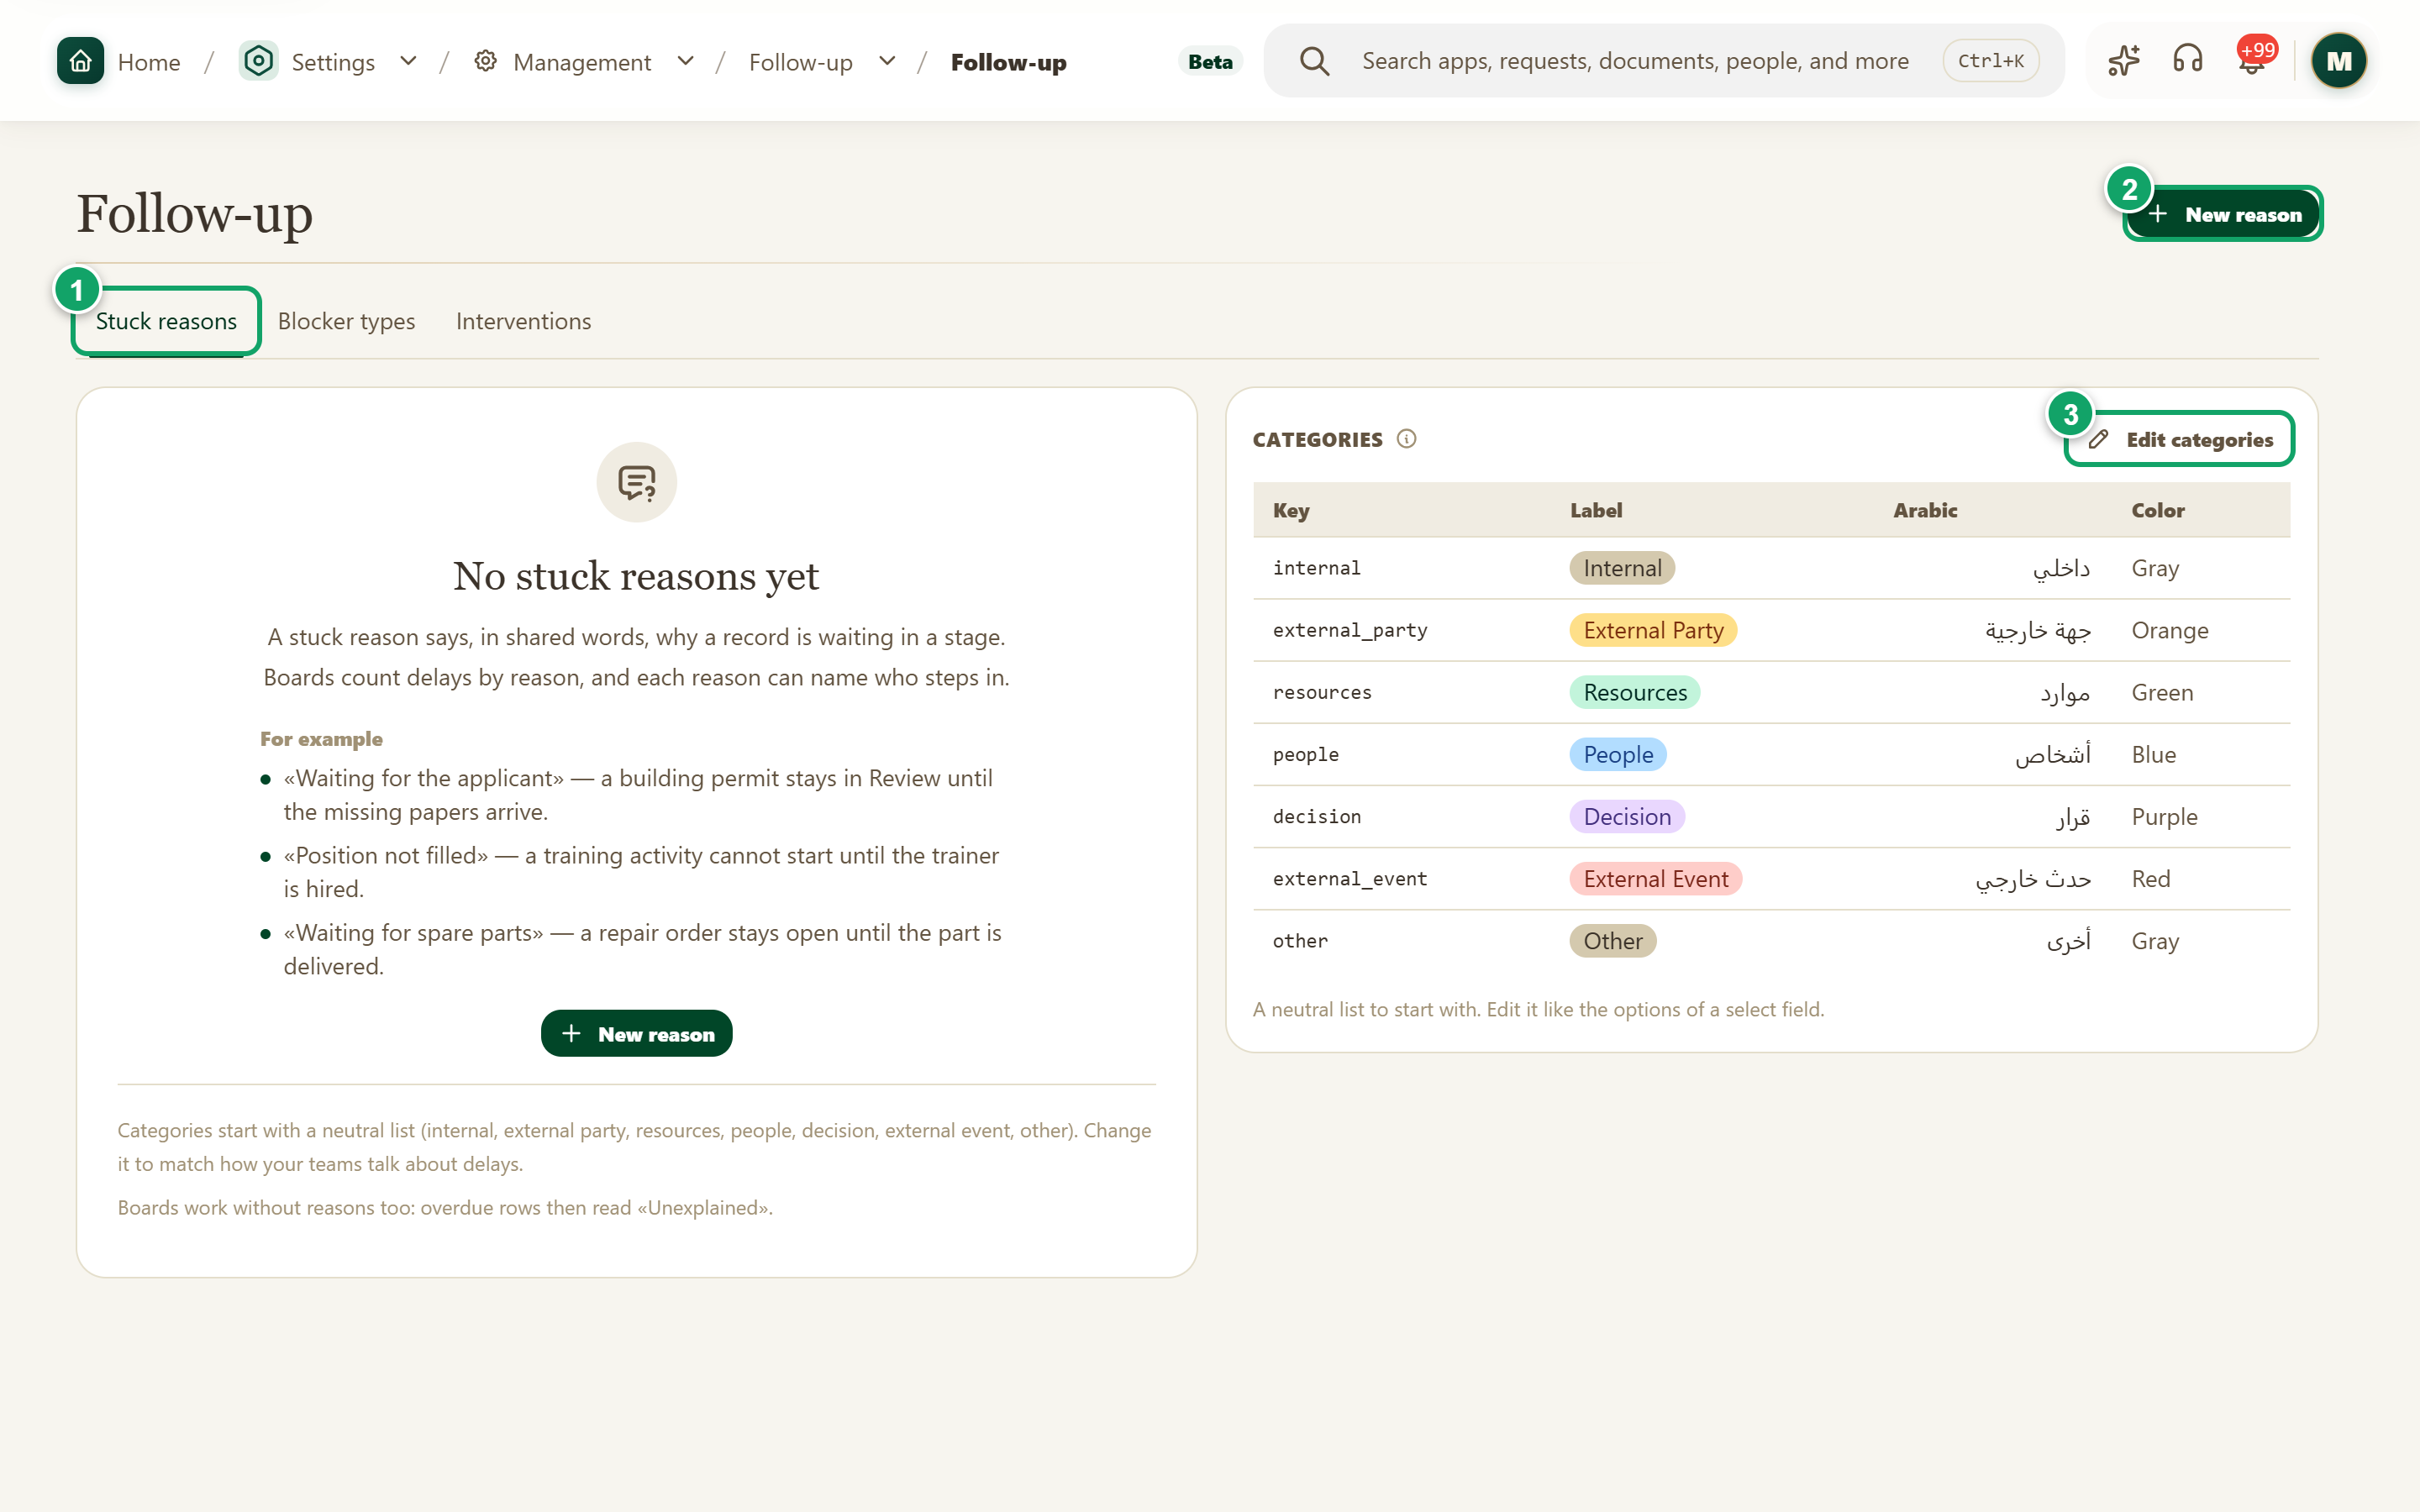
\includegraphics[width=0.95\linewidth,height=0.72\textheight,keepaspectratio]{figures/screens/ch08-followup-en.png}
\caption{Stuck reasons and categories}
\label{fig:settings-followup-screen}
\shotnote{The image shows the empty state of the test organization, which has no reasons yet, beside the category list every organization starts with. Categories group reasons so boards can count delays by cause. ① “Stuck reasons”. ② “New reason”. ③ “Edit categories”.}
\end{figure}

\begin{figure}[H]
\centering
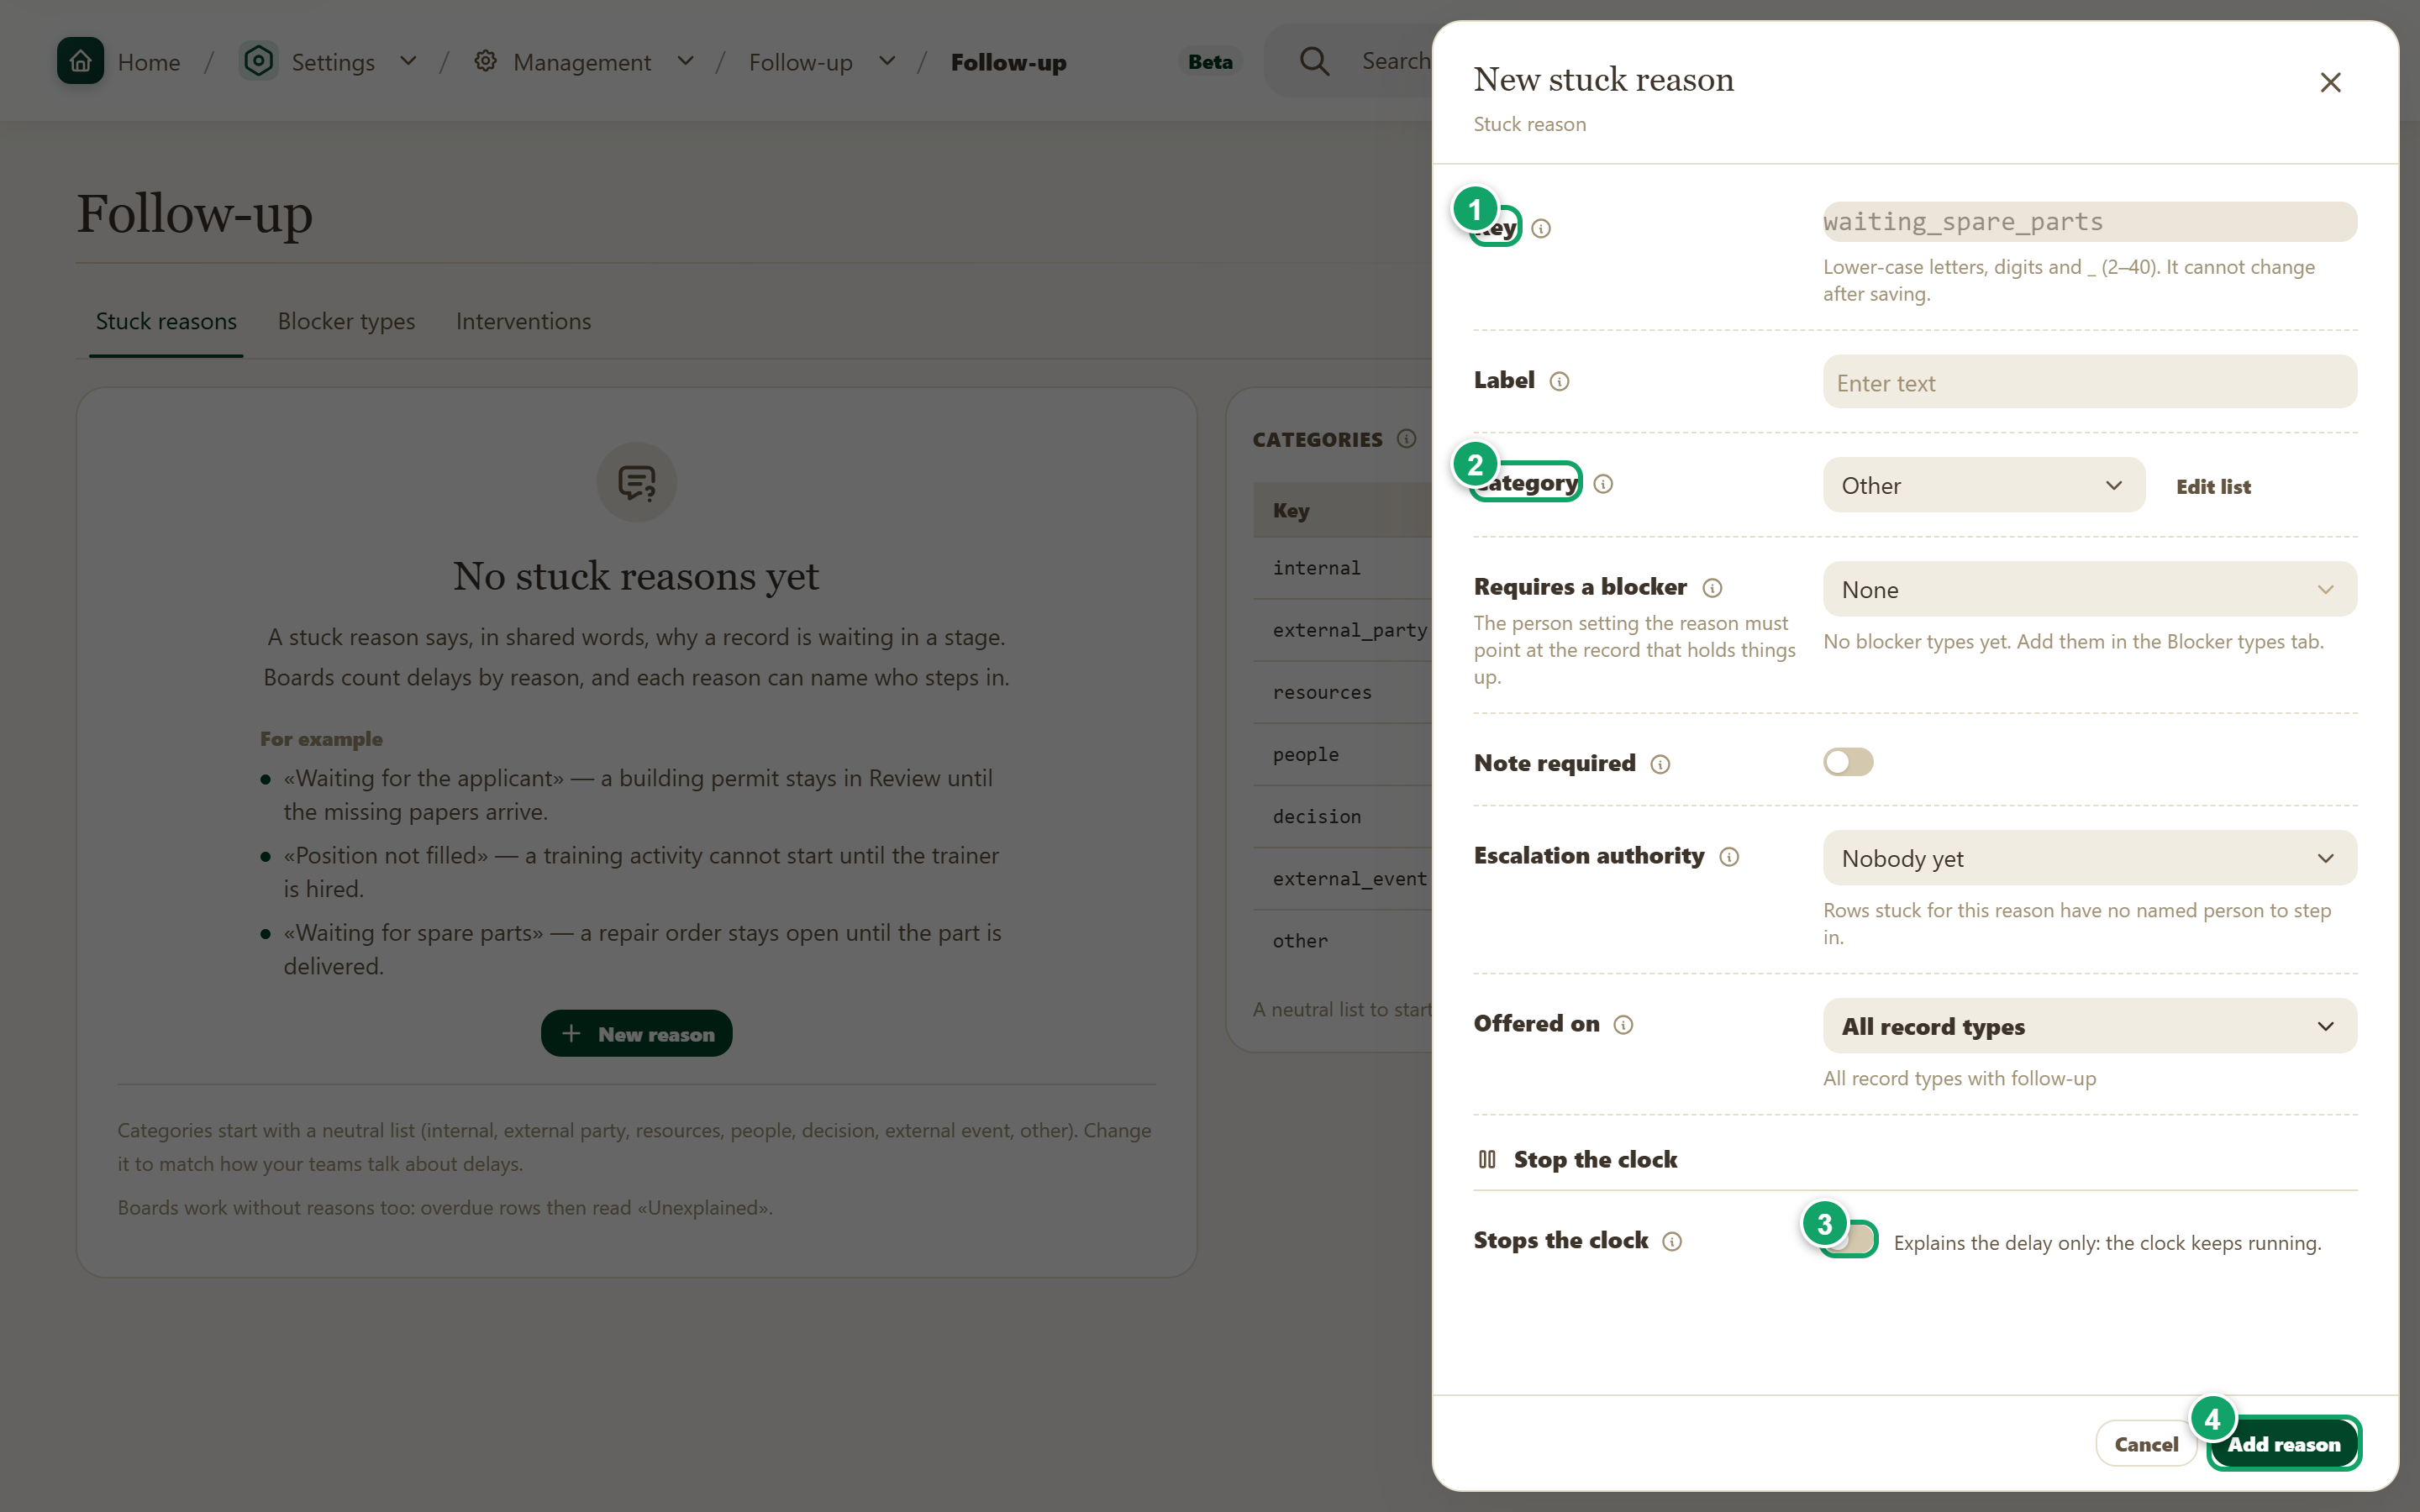
\includegraphics[width=0.95\linewidth,height=0.72\textheight,keepaspectratio]{figures/screens/ch08-followup-reason-en.png}
\caption{The new stuck reason window}
\label{fig:settings-followup-reason-screen}
\shotnote{The window sets what a reason means and how it affects the team’s work. The main decision is the clock: it separates a delay that is only explained from a wait that does not count against the stage. ① “Key”: filled from the label and fixed after saving. ② “Category”. ③ “Stops the clock”: turning it on reveals the resume options and limits. ④ “Add reason”.}
\end{figure}

\begin{figure}[H]
\centering
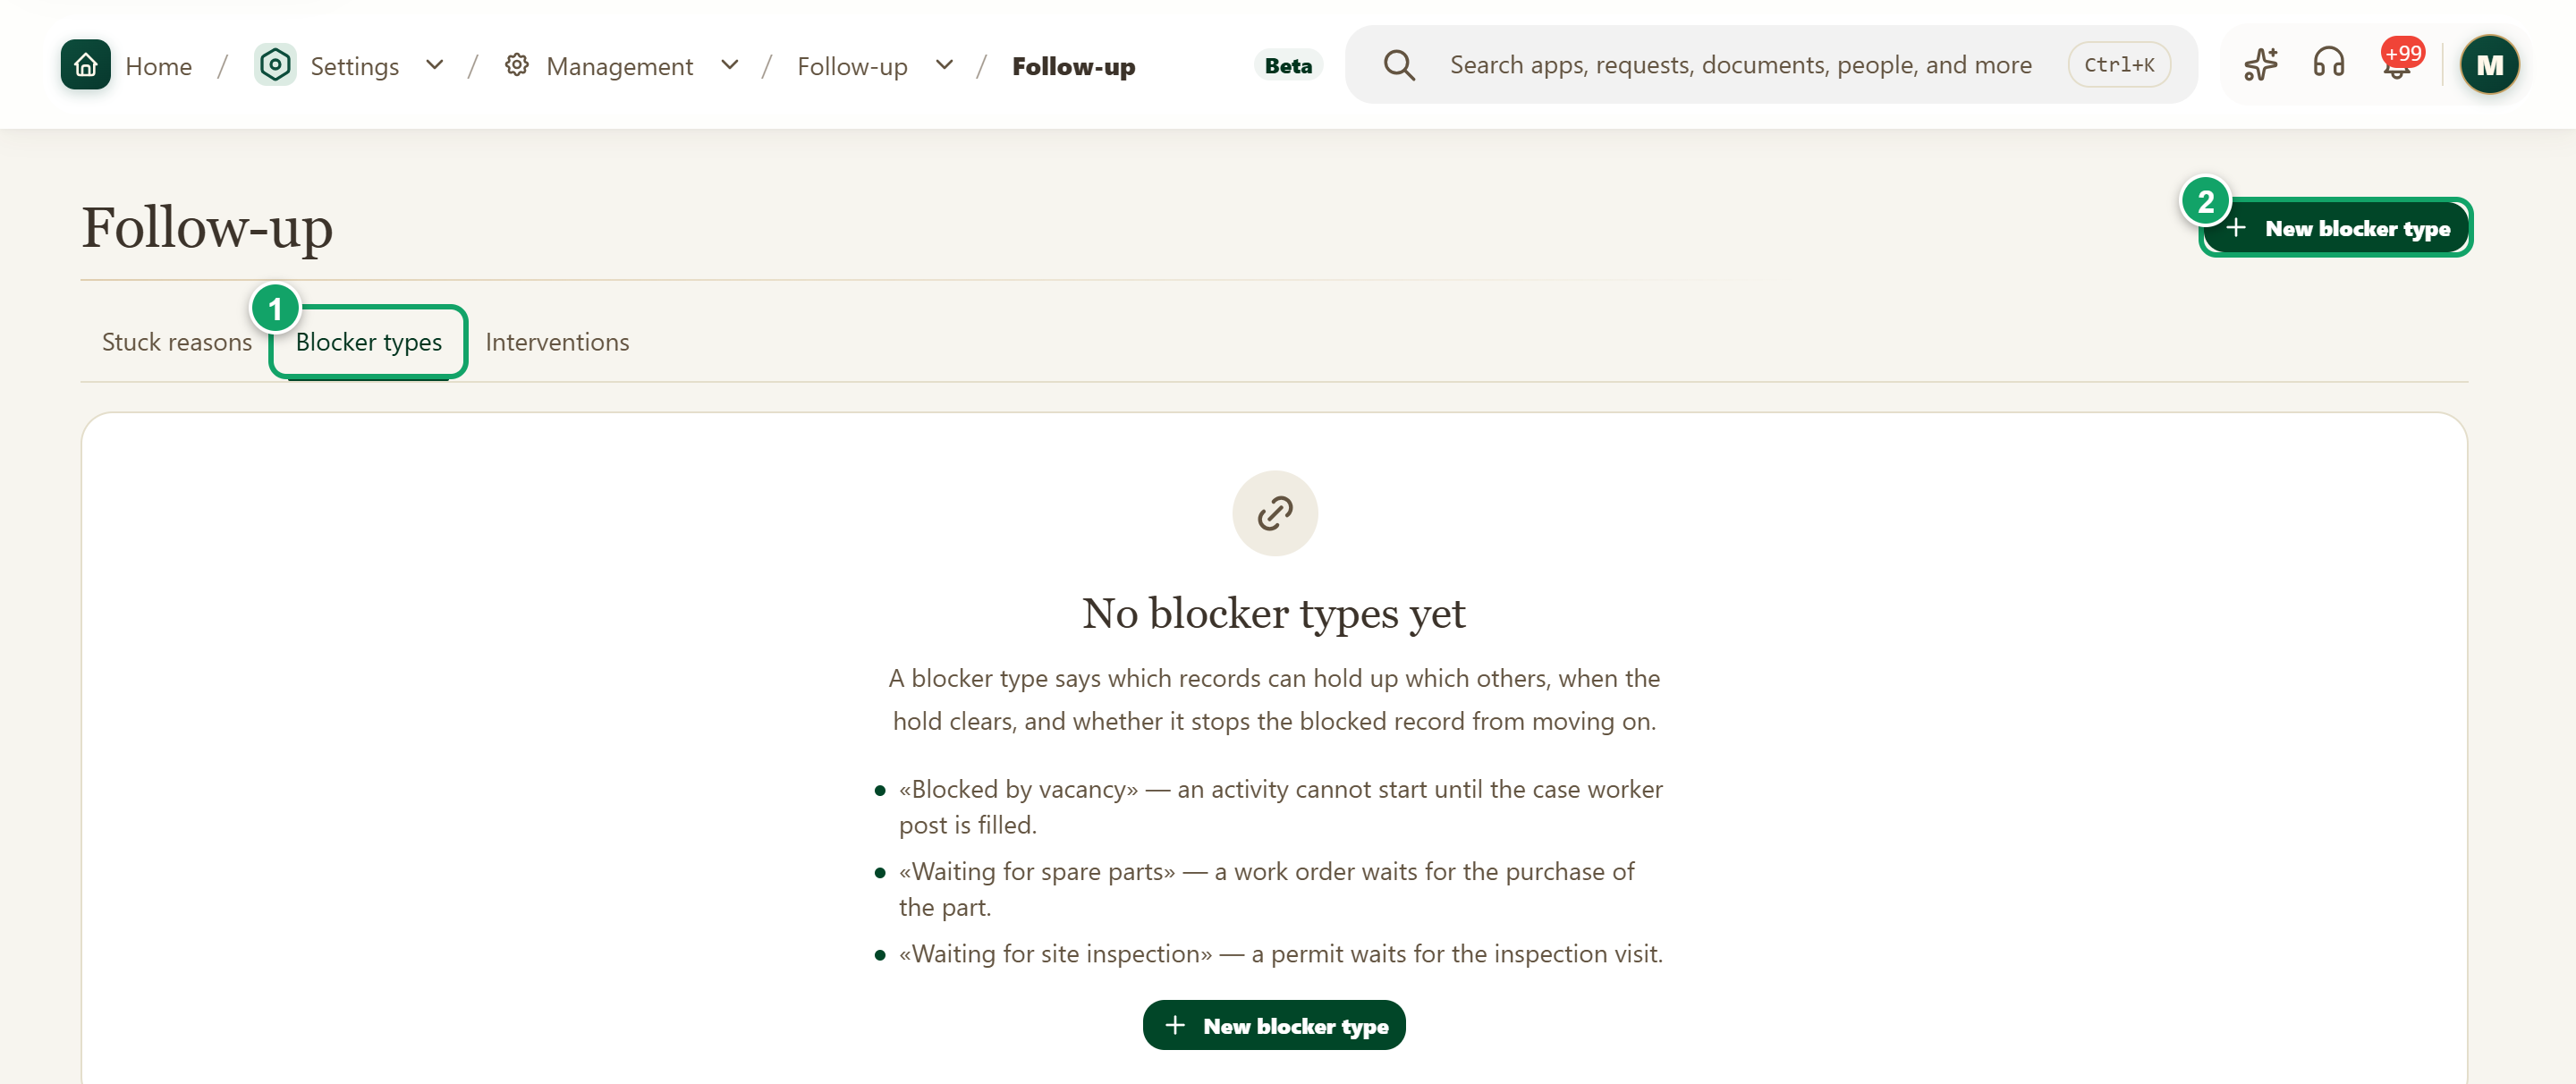
\includegraphics[width=0.95\linewidth,height=0.72\textheight,keepaspectratio]{figures/screens/ch08-followup-blockers-en.png}
\caption{Blocker types}
\label{fig:settings-followup-blockers-screen}
\shotnote{A blocker type sets which records can hold up others, when the hold clears, and whether it stops the record from moving on. The tab is empty in the test organization, so the image shows the explanation and examples the system offers. ① “Blocker types”. ② “New blocker type”.}
\end{figure}

\begin{figure}[H]
\centering
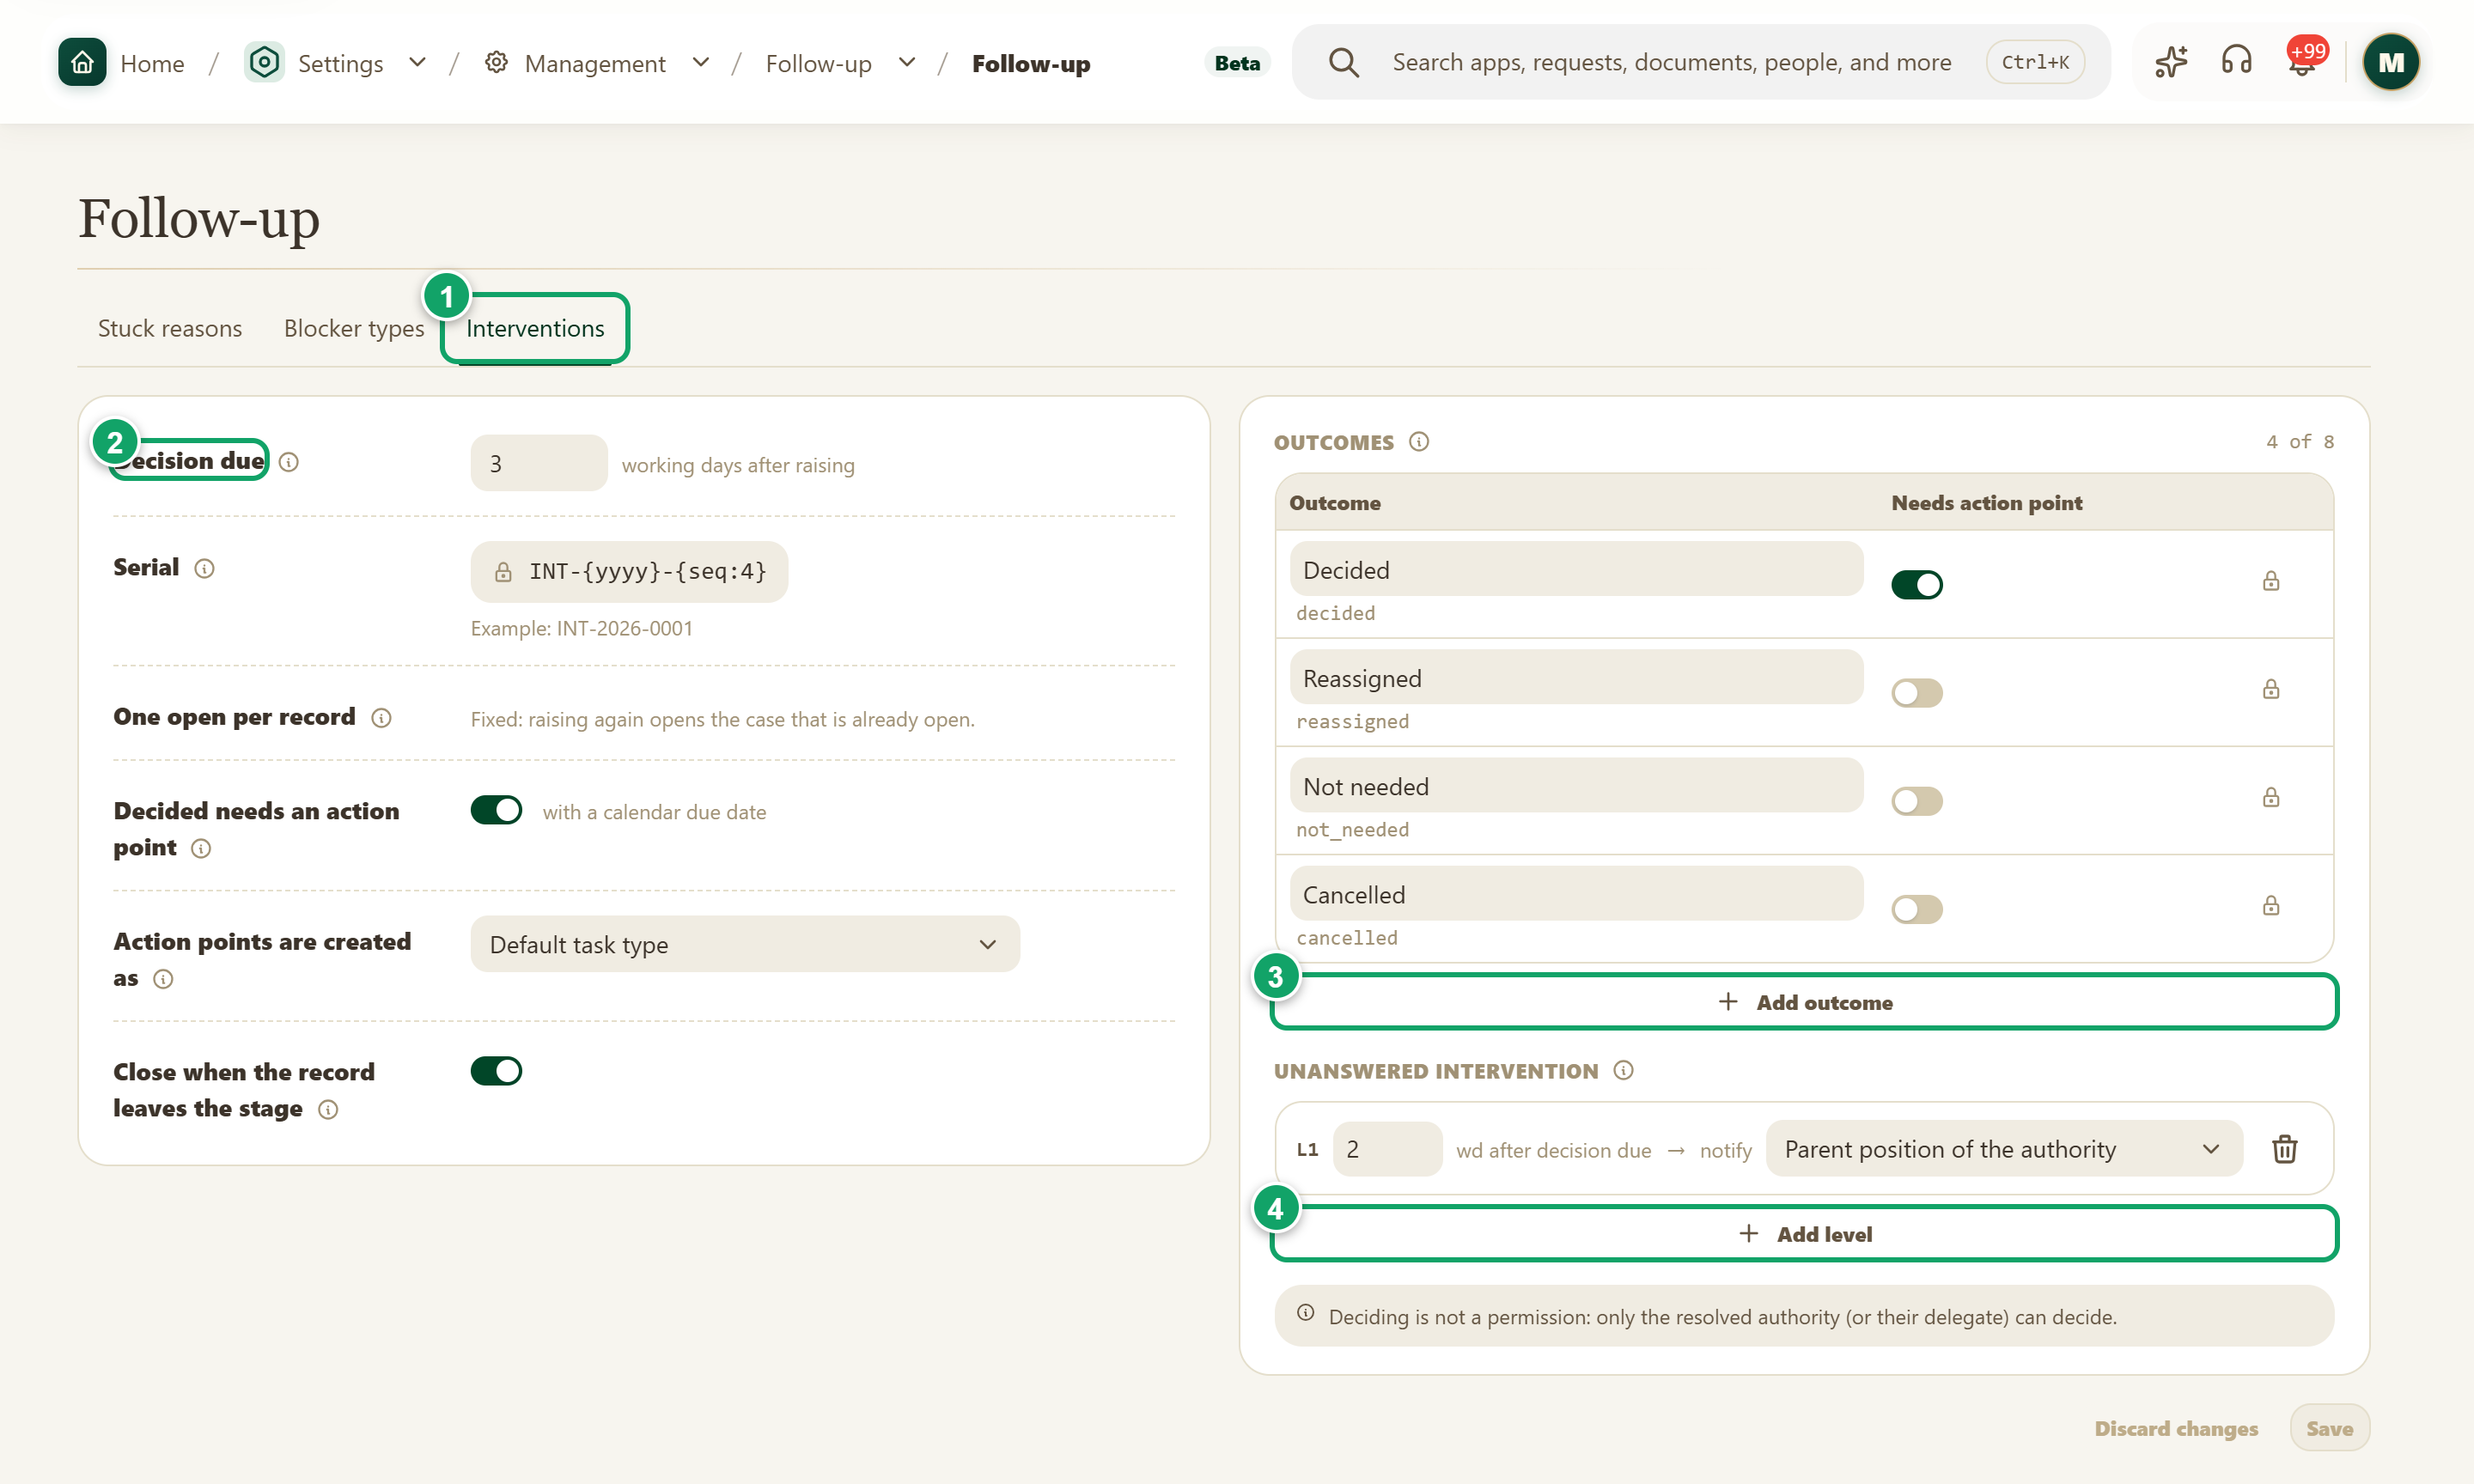
\includegraphics[width=0.95\linewidth,height=0.72\textheight,keepaspectratio]{figures/screens/ch08-followup-interventions-en.png}
\caption{Intervention settings}
\label{fig:settings-followup-interventions-screen}
\shotnote{This tab sets the deadline for deciding an intervention, the outcomes that can be recorded, and who is told if nothing is decided. Deciding itself is not a permission you grant: only the named authority or their delegate can decide. ① “Interventions”. ② “Decision due”. ③ “Add outcome”. ④ “Add level”: adds a notification step after the decision date.}
\end{figure}

\begin{table}[H]
\centering
\caption{What do you record in each tab?}
\label{tab:settings-followup-fields}
\begin{tabularx}{\linewidth}{R{4.2cm} Y}
\rcHeaderRow
\thh{Tab} & \thh{What you record there}\\
“Stuck reasons” & “Key”, “Label”, “Category”, “Requires a blocker”, “Note required”, “Escalation authority” and “Offered on”. With “Stops the clock”, you also set the resume events, the wait limit, and what the other party sees in their portal.\\
“Blocker types” & “Key”, “Forward label” and “Inverse label”, “Can be blocked” and “Can block”, when the blocker clears, and “Effect on the blocked record”: “Show only”, “Warn” or “Refuse”.\\
“Interventions” & “Decision due”, “Serial”, “Decided needs an action point”, “Action points are created as”, “Close when the record leaves the stage”, “Outcomes” and “Unanswered intervention”.\\
“SLA calendars” & Appears only when the Cases module is on, and did not appear in the test organization. It sets working days and hours, holidays and dated exceptions.\\
\end{tabularx}
\end{table}

\begin{enumerate}
\item Open “Settings”, then “Follow-up”.
\item Press “Edit categories” if you want the categories to match how your team talks about delays, then save them.
\item Press “New reason”, enter “Label”, choose “Category”, set any options you need, and press “Add reason”.
\item Create blocker types in their tab if you need to link records, then review “Interventions” and press “Save”.
\item To remove an unused reason, open it, press “Delete” and confirm. A reason that has been used can only be archived, so history keeps its words.
\end{enumerate}

\textbf{Check:} The reason appears in the “Active” table with zero in the “Used” column, and stays after you reload the page. After you delete an unused reason, the message “Reason deleted” appears and it leaves the table. At the limit of 60 active reasons, archive one before adding another.

\section{Record keeping}
\label{sec:settings-feature-record-keeping}

This page manages the life of important records after work on them ends. Four terms help: “retention” is how long a record stays before anything is done with it; “declaring” a record makes it an official record; a “hold” stops records linked to a case or audit from being deleted or disposed of; and “disposition” is the final action on a record when its period ends, whether deleting it, anonymizing it or transferring it. The page opens for those holding the Records officer, Legal affairs, disposition approver or Records reader role. Record keeping is turned on per record type in the Builder; this page shows it across the organization.

\begin{rcnote}[Example: Horizon]
The system administrator sets supplier contracts to be kept for seven years after they are declared. When a dispute arises with a supplier, the holder of the Legal affairs role places a hold on that supplier’s contracts, so they stay out of disposition reviews until the hold is released.
\end{rcnote}

\begin{figure}[H]
\centering
\begin{tikzpicture}[node distance=0.5cm]
\node[stepBox] (a) {Retention starts at the chosen event};
\node[stepBox,below=of a] (b) {The period ends and the record is due};
\node[stepBox,below=of b] (c) {A disposition review is proposed};
\node[stepBox,below=of c] (d) {Records on hold are left out};
\node[stepBox,below=of d] (e) {Two or more different people approve};
\node[stepBox,below=of e] (f) {The system acts and issues a signed certificate};
\draw[flowsTo] (a) -- (b);
\draw[flowsTo] (b) -- (c);
\draw[flowsTo] (c) -- (d);
\draw[flowsTo] (d) -- (e);
\draw[flowsTo] (e) -- (f);
\end{tikzpicture}
\rclegend
\caption{A record’s journey from retention to disposition}
\label{fig:settings-record-keeping-journey}
\shotnote{The diagram shows that the end of a period does not remove a record at once: people must review and approve before anything happens. This journey does not apply to a keep-permanently rule, and holds are checked again before the action runs.}
\end{figure}

\begin{figure}[H]
\centering
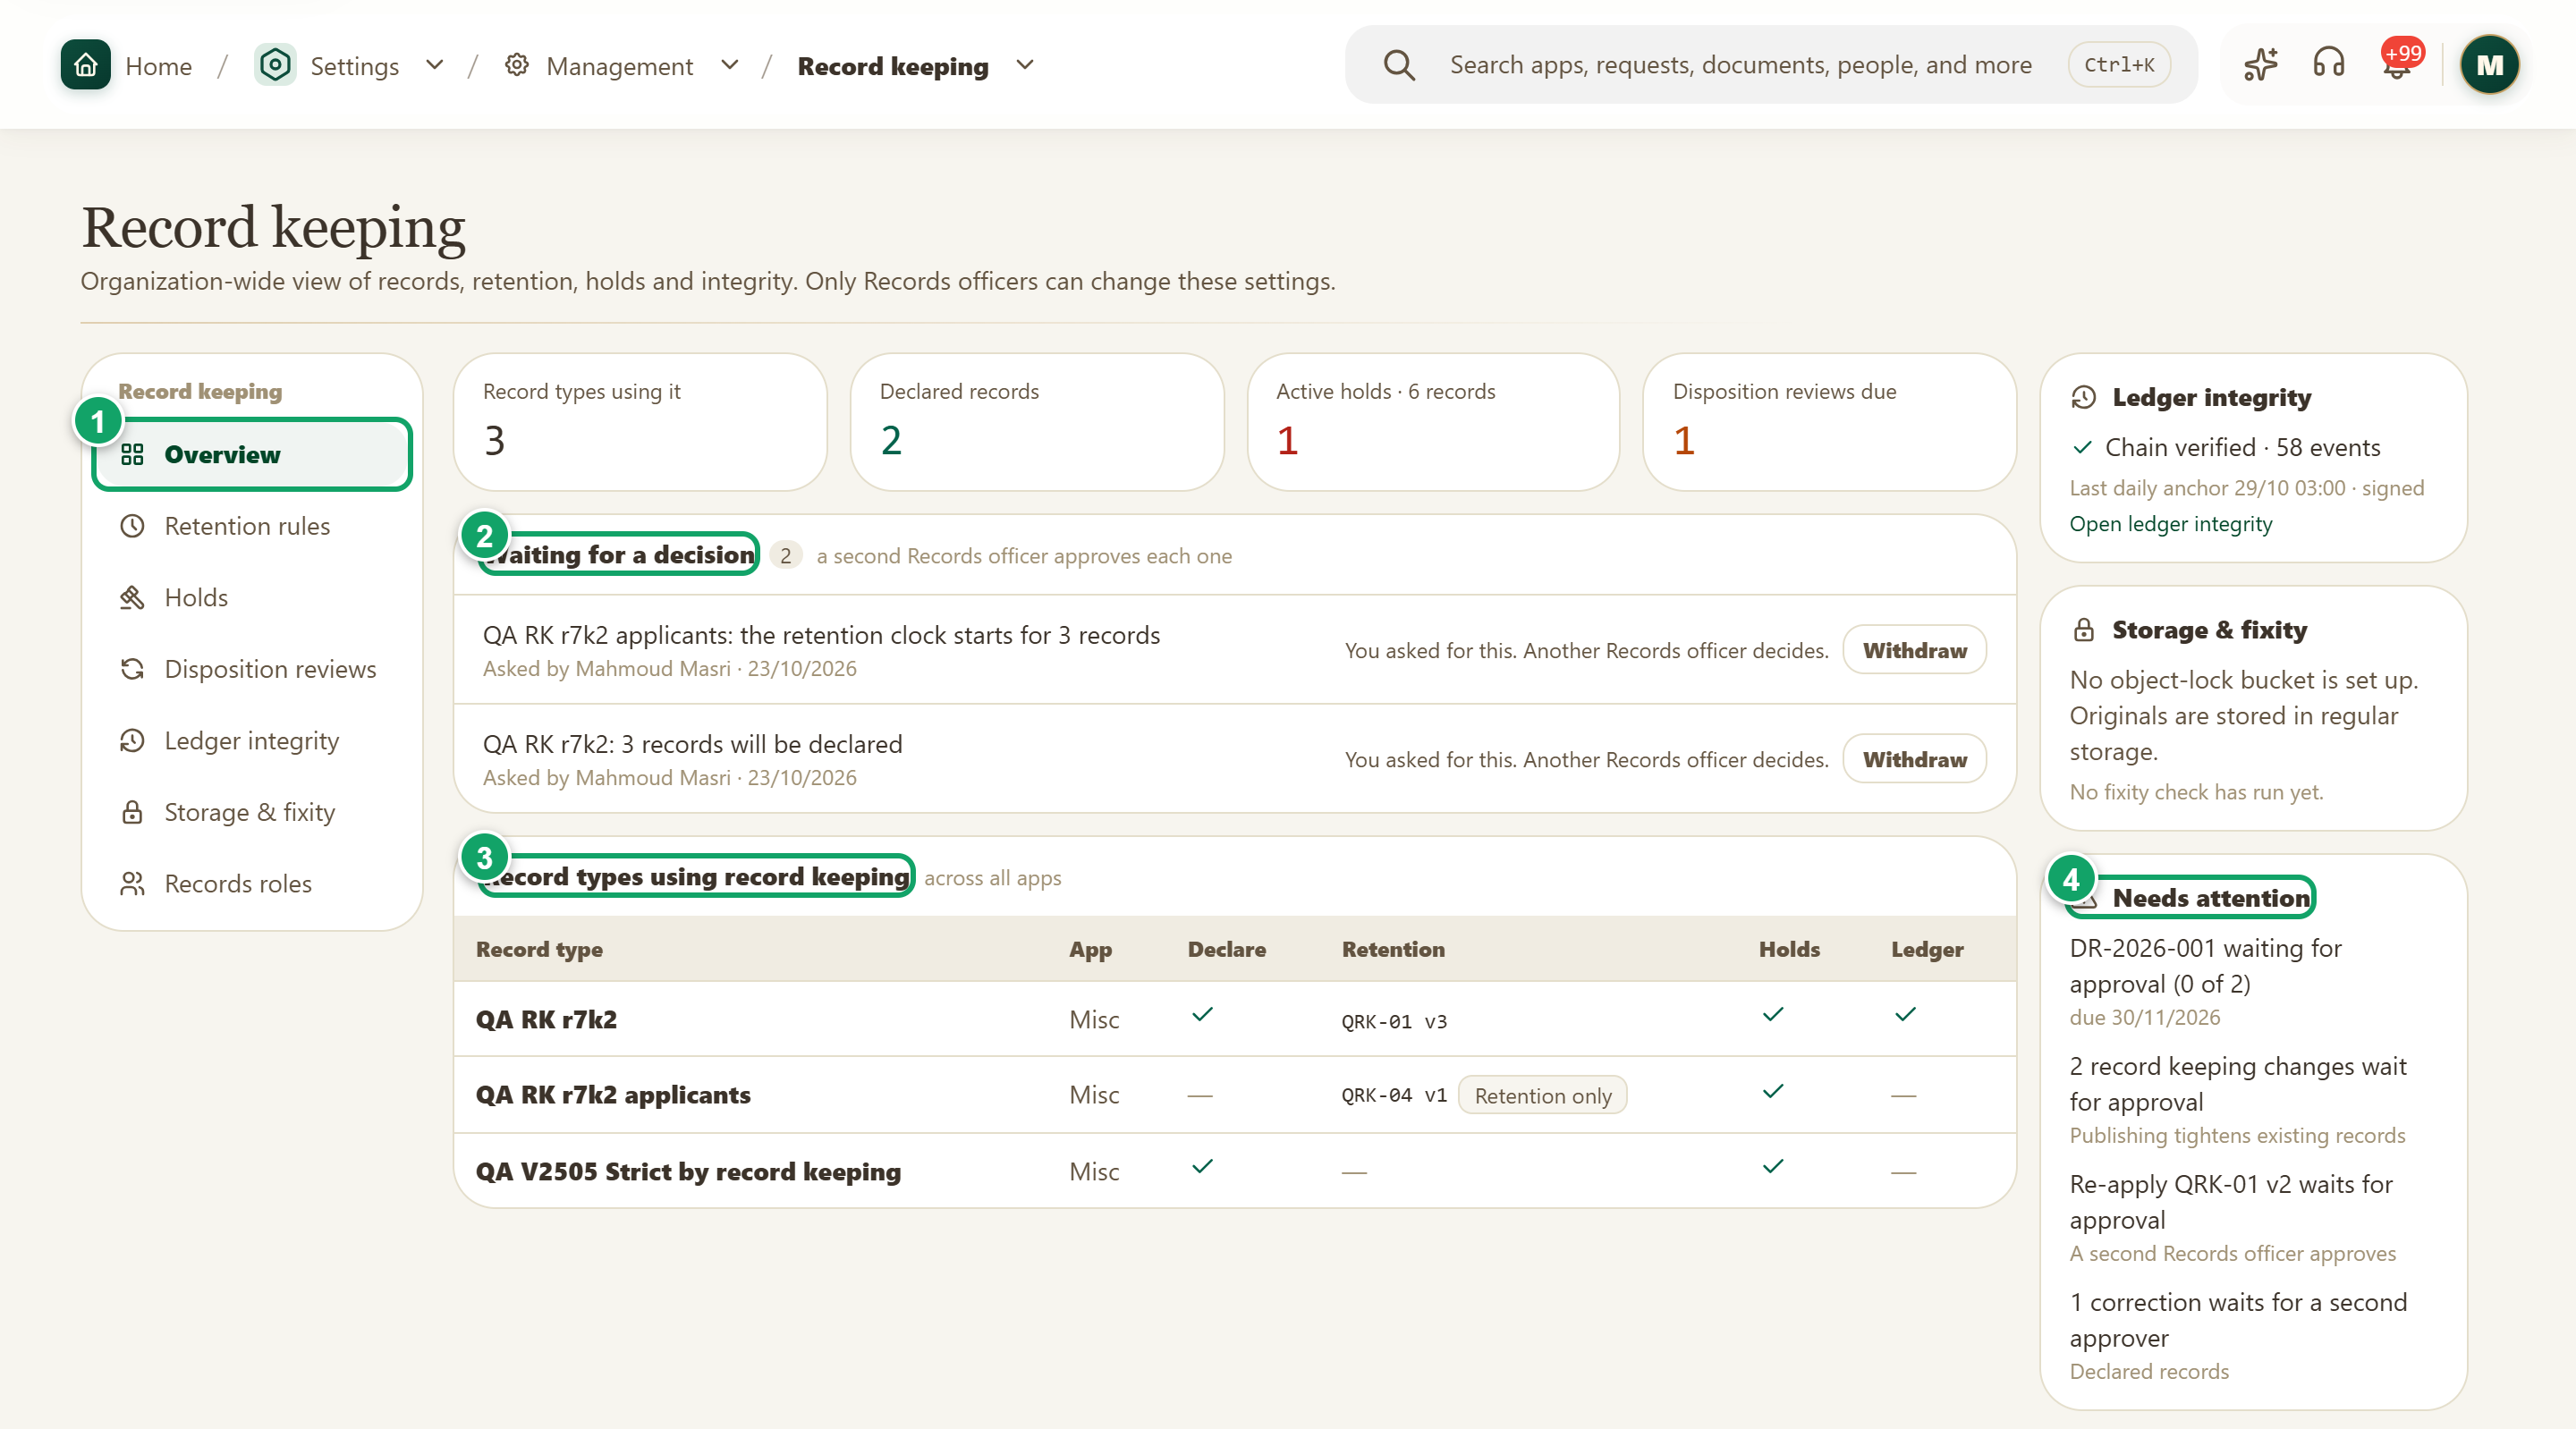
\includegraphics[width=0.95\linewidth,height=0.72\textheight,keepaspectratio]{figures/screens/ch08-record-keeping-en.png}
\caption{Record keeping overview}
\label{fig:settings-record-keeping-screen}
\shotnote{The overview gathers the main figures and what awaits a decision, so you know where to start. The data shown is test data. A requester cannot approve their own request, so the row says it waits for another Records officer. ① “Overview”. ② “Waiting for a decision”. ③ “Record types using record keeping”. ④ “Needs attention”.}
\end{figure}

\begin{figure}[H]
\centering
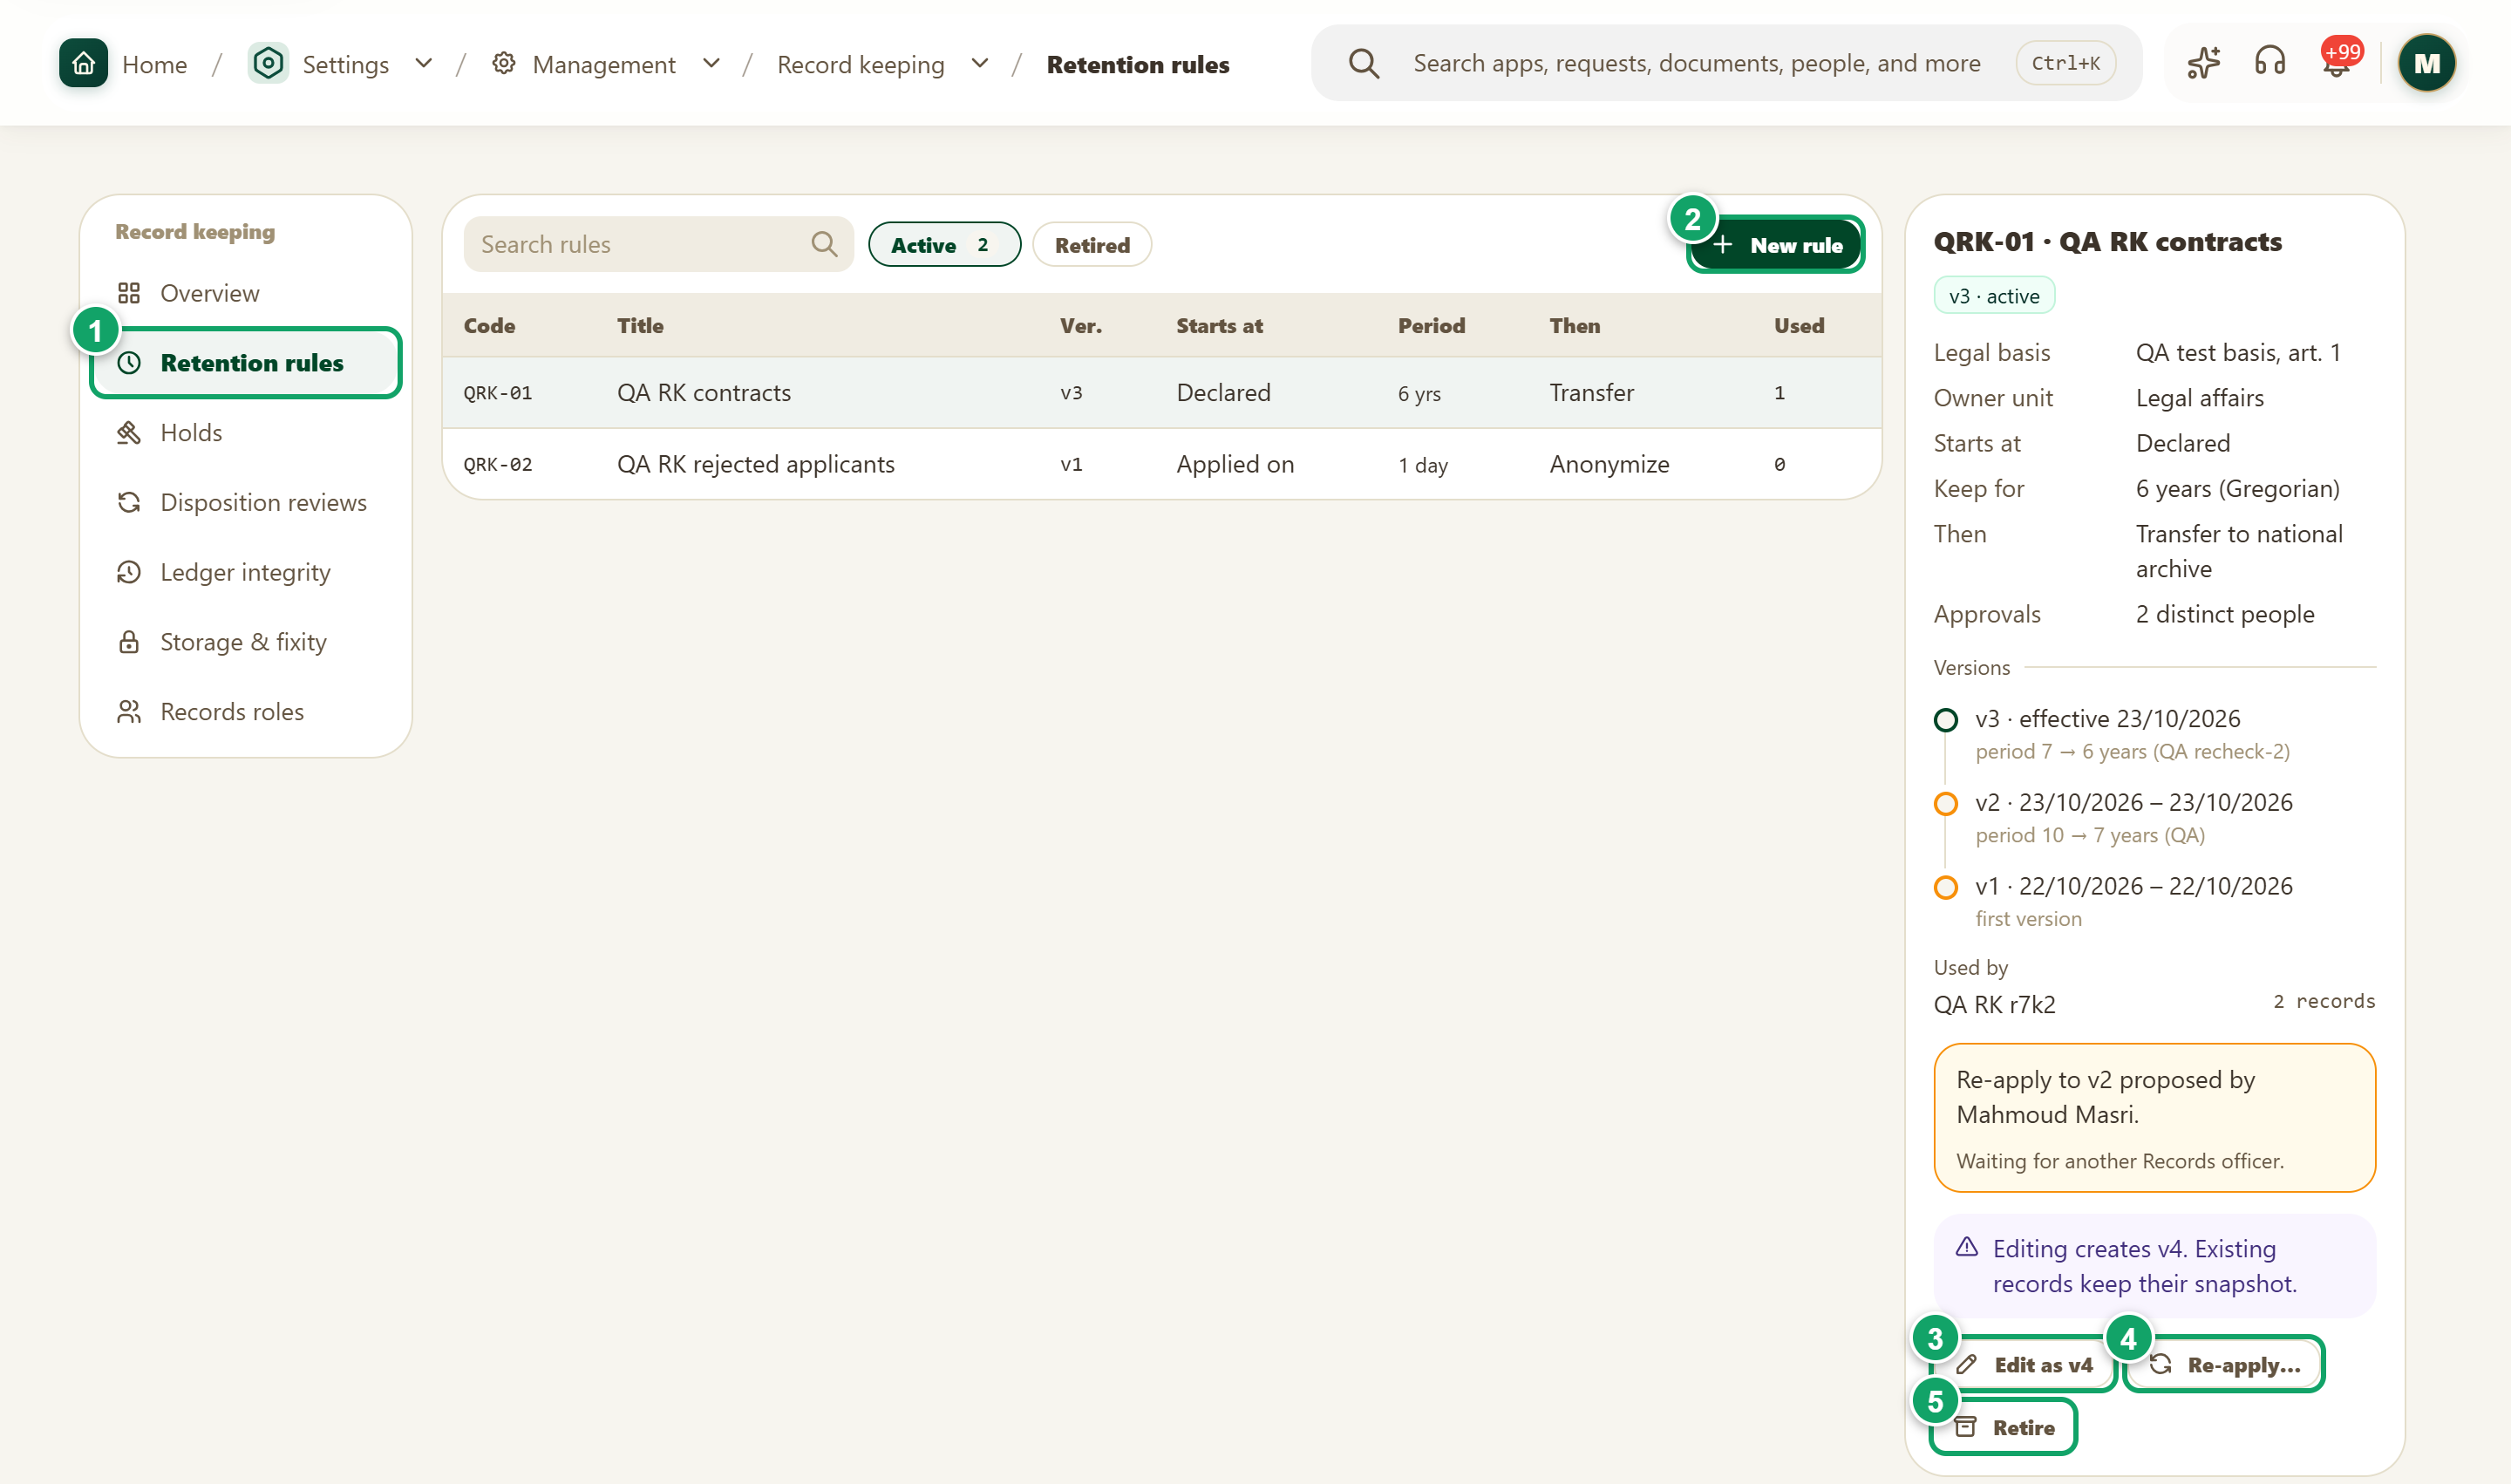
\includegraphics[width=0.95\linewidth,height=0.72\textheight,keepaspectratio]{figures/screens/ch08-record-keeping-rules-en.png}
\caption{Retention rules}
\label{fig:settings-record-keeping-rules-screen}
\shotnote{A rule sets when the period starts, how long it runs and what happens next. Editing creates a new version, and existing records keep theirs until a re-apply is approved. ① “Retention rules”. ② “New rule”. ③ “Edit as v…”. ④ “Re-apply…”: proposes moving existing records; another Records officer approves it. ⑤ “Retire”: new records can no longer use the rule.}
\end{figure}

\begin{figure}[H]
\centering
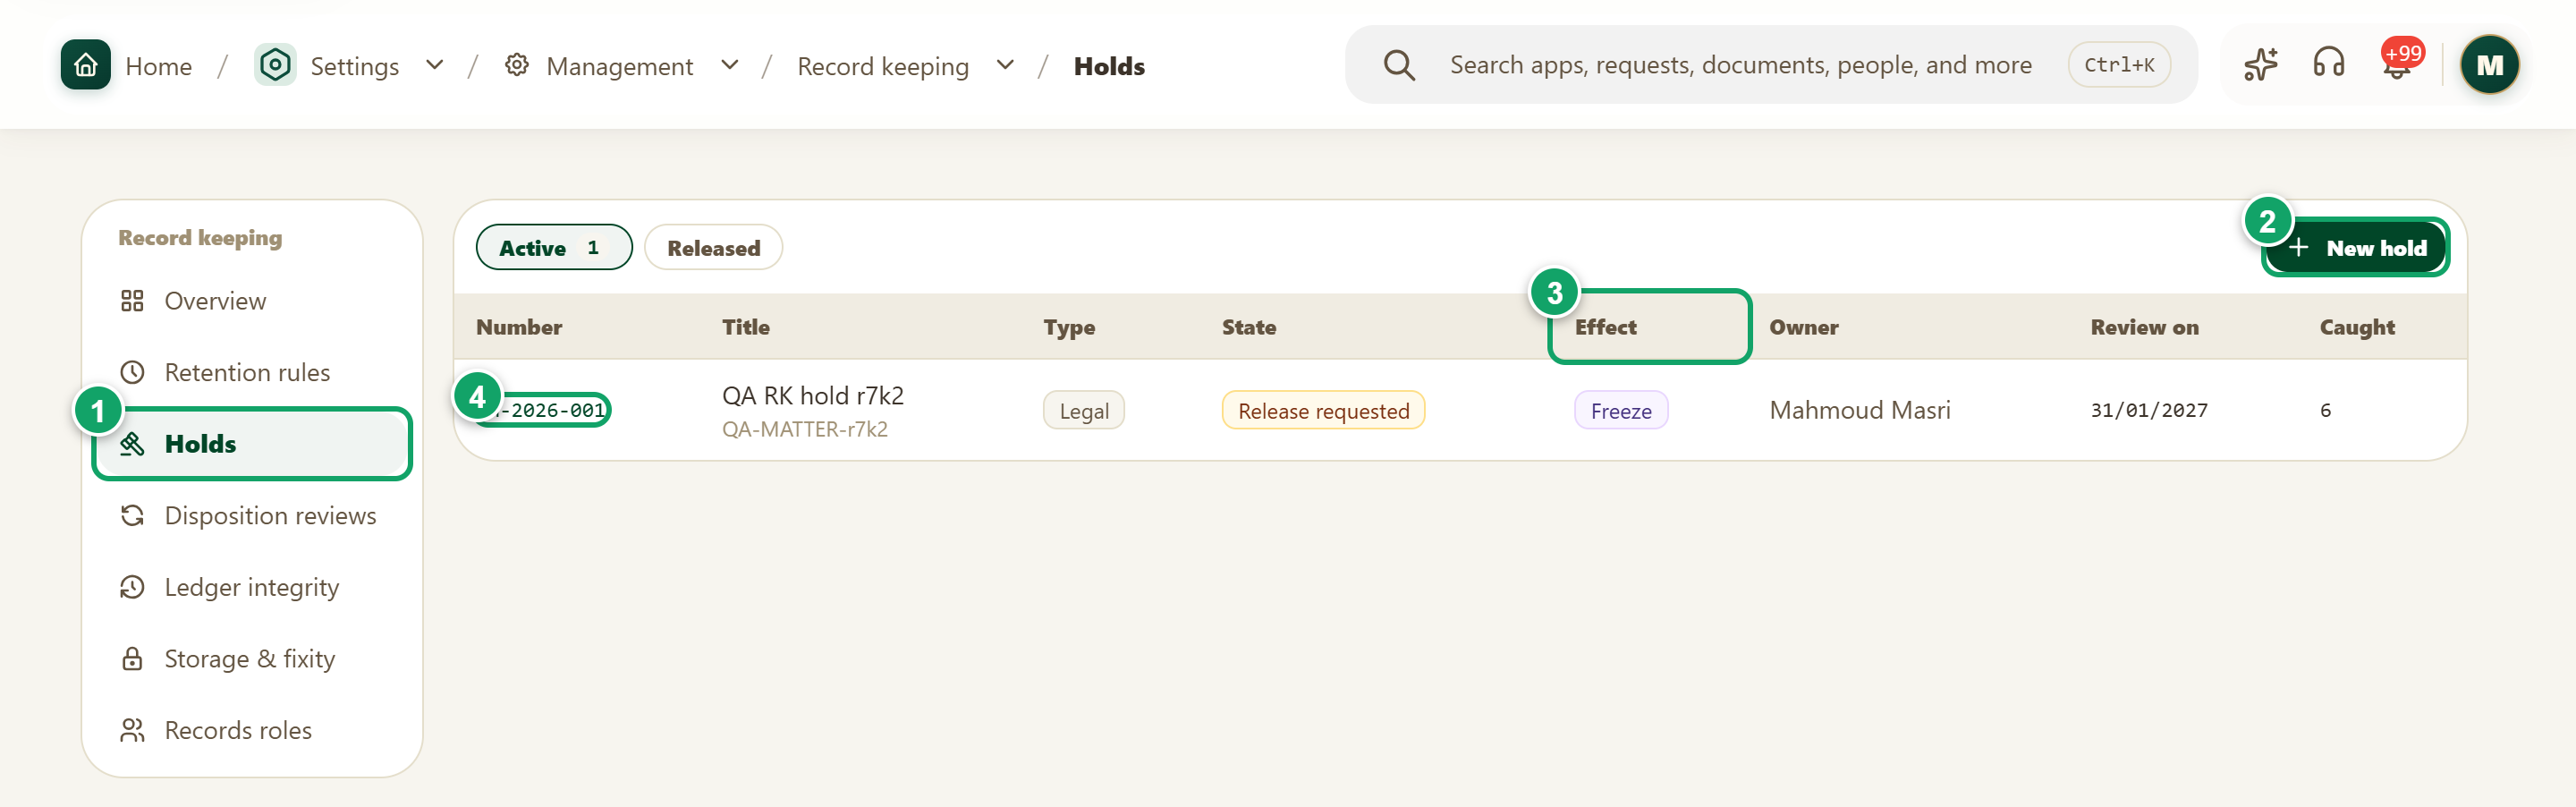
\includegraphics[width=0.95\linewidth,height=0.72\textheight,keepaspectratio]{figures/screens/ch08-record-keeping-holds-en.png}
\caption{Holds}
\label{fig:settings-record-keeping-holds-screen}
\shotnote{A hold suspends disposition and deletion for chosen records, and its scope is checked again nightly and on every change. It is released only with the agreement of Legal affairs and the hold owner. ① “Holds”. ② “New hold”. ③ “Effect”: “Preserve” allows edits and keeps every version; “Freeze” stops edits too. ④ The hold number: opens its scope and records.}
\end{figure}

\begin{figure}[H]
\centering
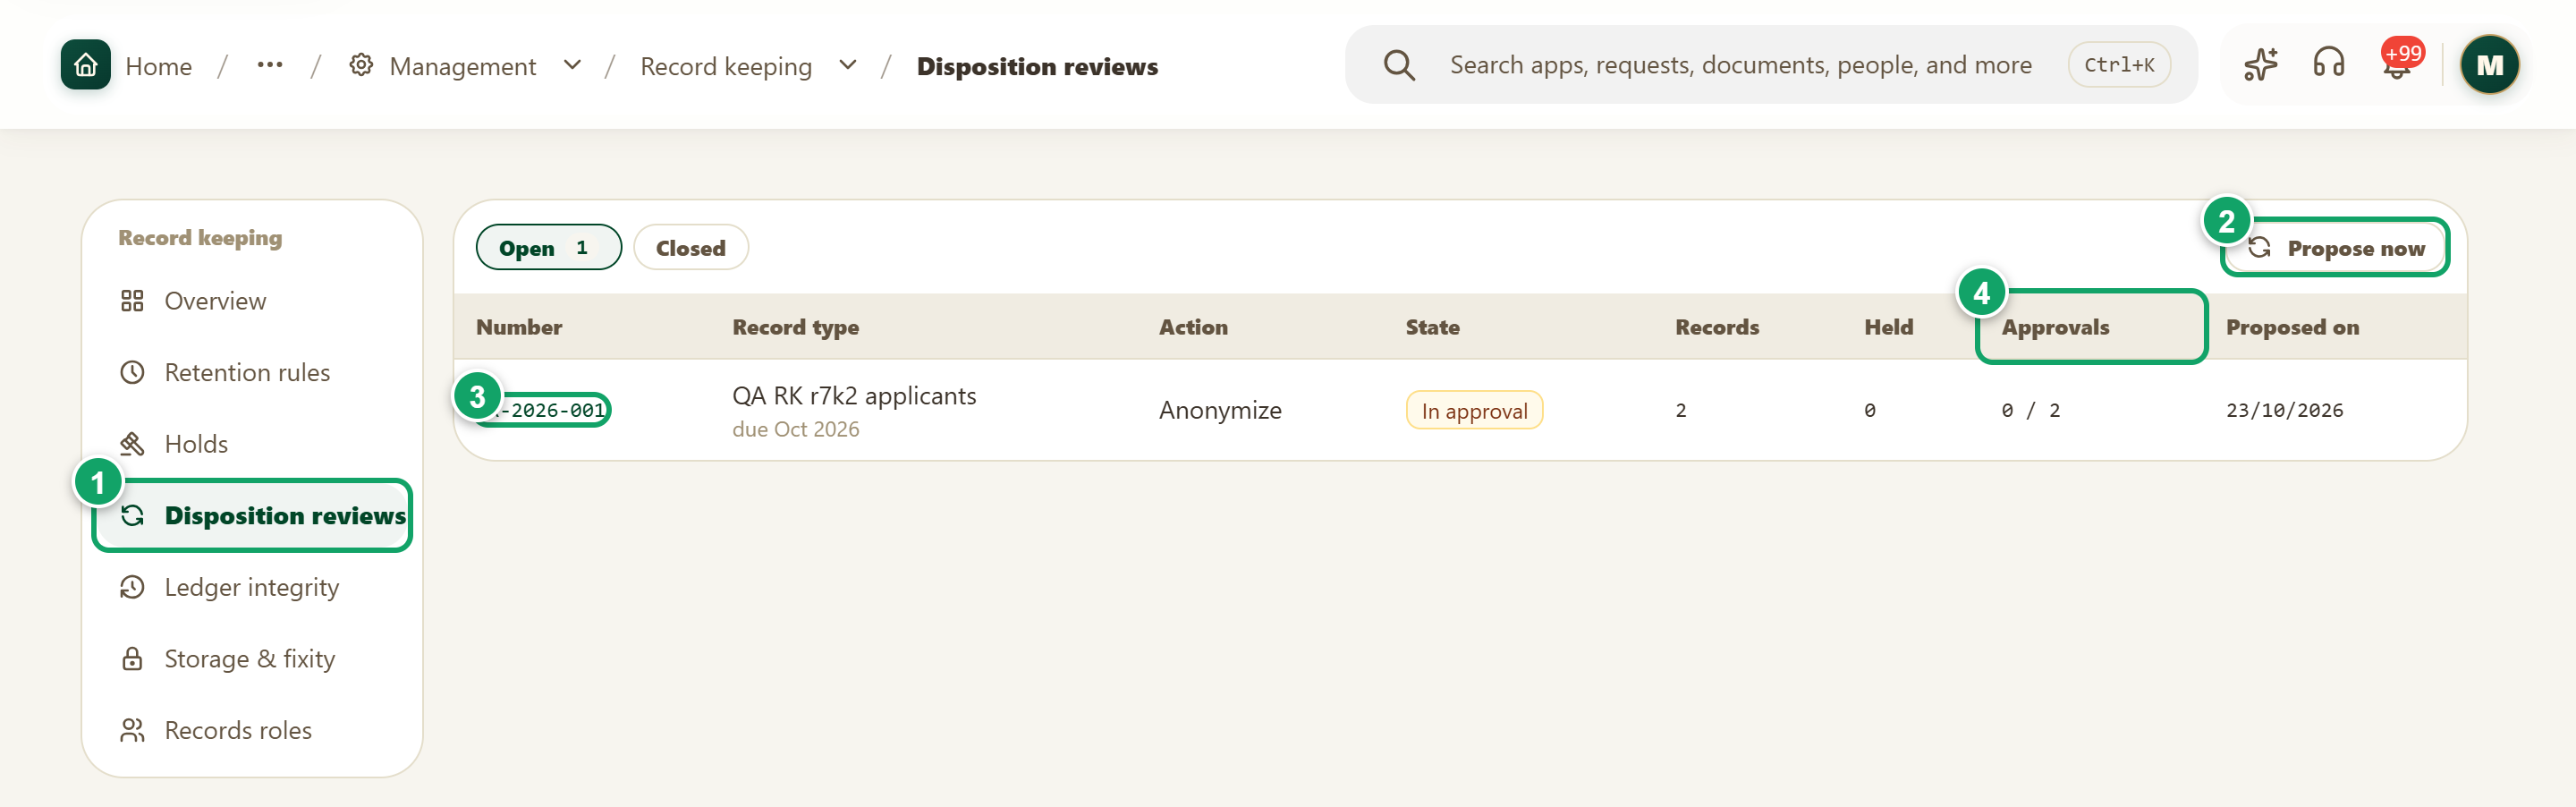
\includegraphics[width=0.95\linewidth,height=0.72\textheight,keepaspectratio]{figures/screens/ch08-record-keeping-disposition-en.png}
\caption{Disposition reviews}
\label{fig:settings-record-keeping-disposition-screen}
\shotnote{A review gathers the due records into one request that must be approved before anything runs. The system proposes reviews monthly, and whoever proposes one cannot approve it. ① “Disposition reviews”. ② “Propose now”: creates the due reviews without waiting for the monthly run. ③ The review number: opens its records, approvals and certificate. ④ “Approvals”.}
\end{figure}

\begin{figure}[H]
\centering
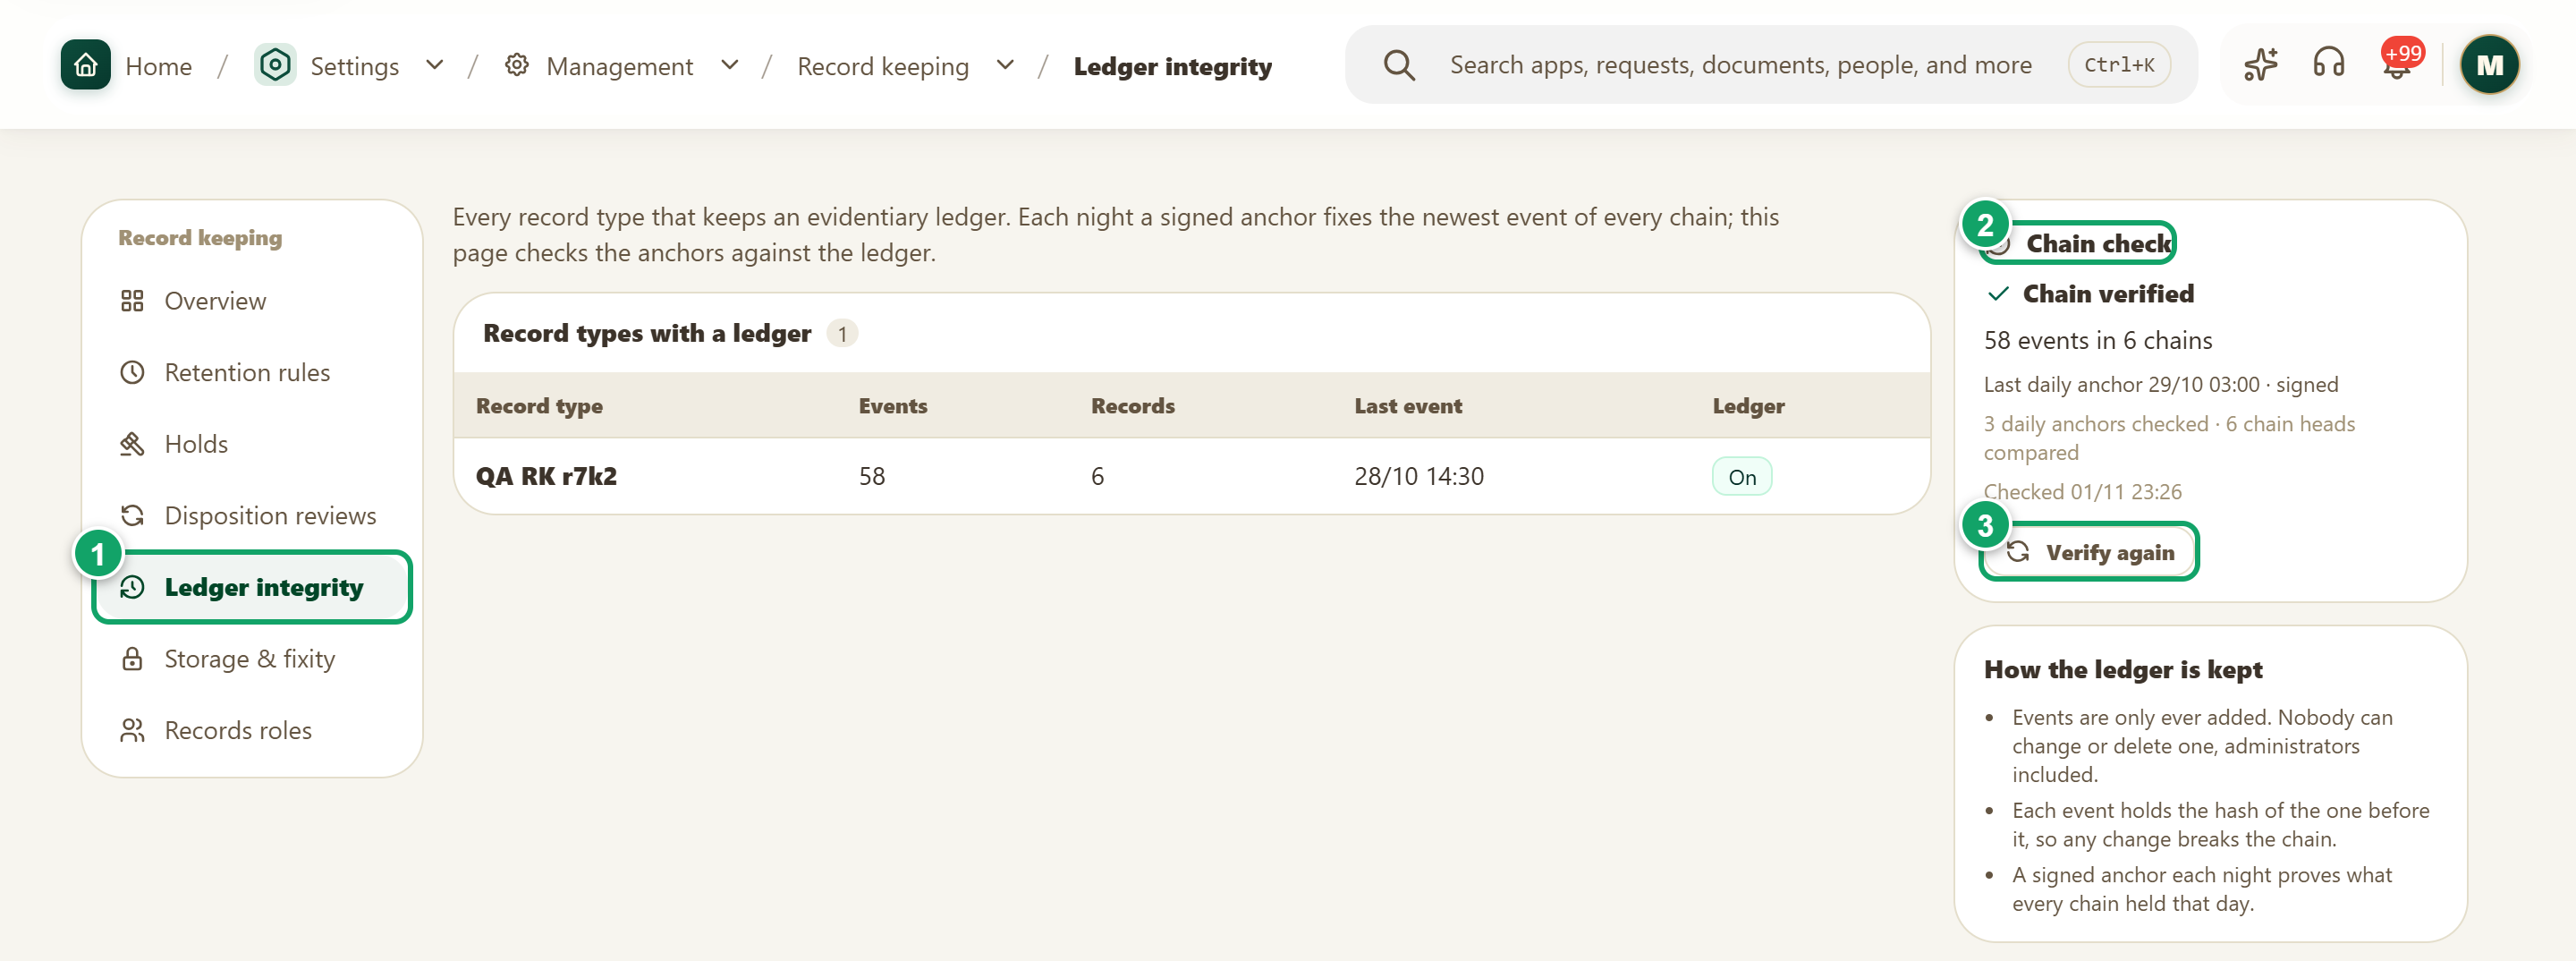
\includegraphics[width=0.95\linewidth,height=0.72\textheight,keepaspectratio]{figures/screens/ch08-record-keeping-ledger-en.png}
\caption{Ledger integrity}
\label{fig:settings-record-keeping-ledger-screen}
\shotnote{The ledger is a list of events that nobody can delete or change, administrators included. Each event is chained to the one before, so any tampering shows up in the check. ① “Ledger integrity”. ② “Chain check”: shows the comparison with the signed reference points saved each night. ③ “Verify again”.}
\end{figure}

\begin{figure}[H]
\centering
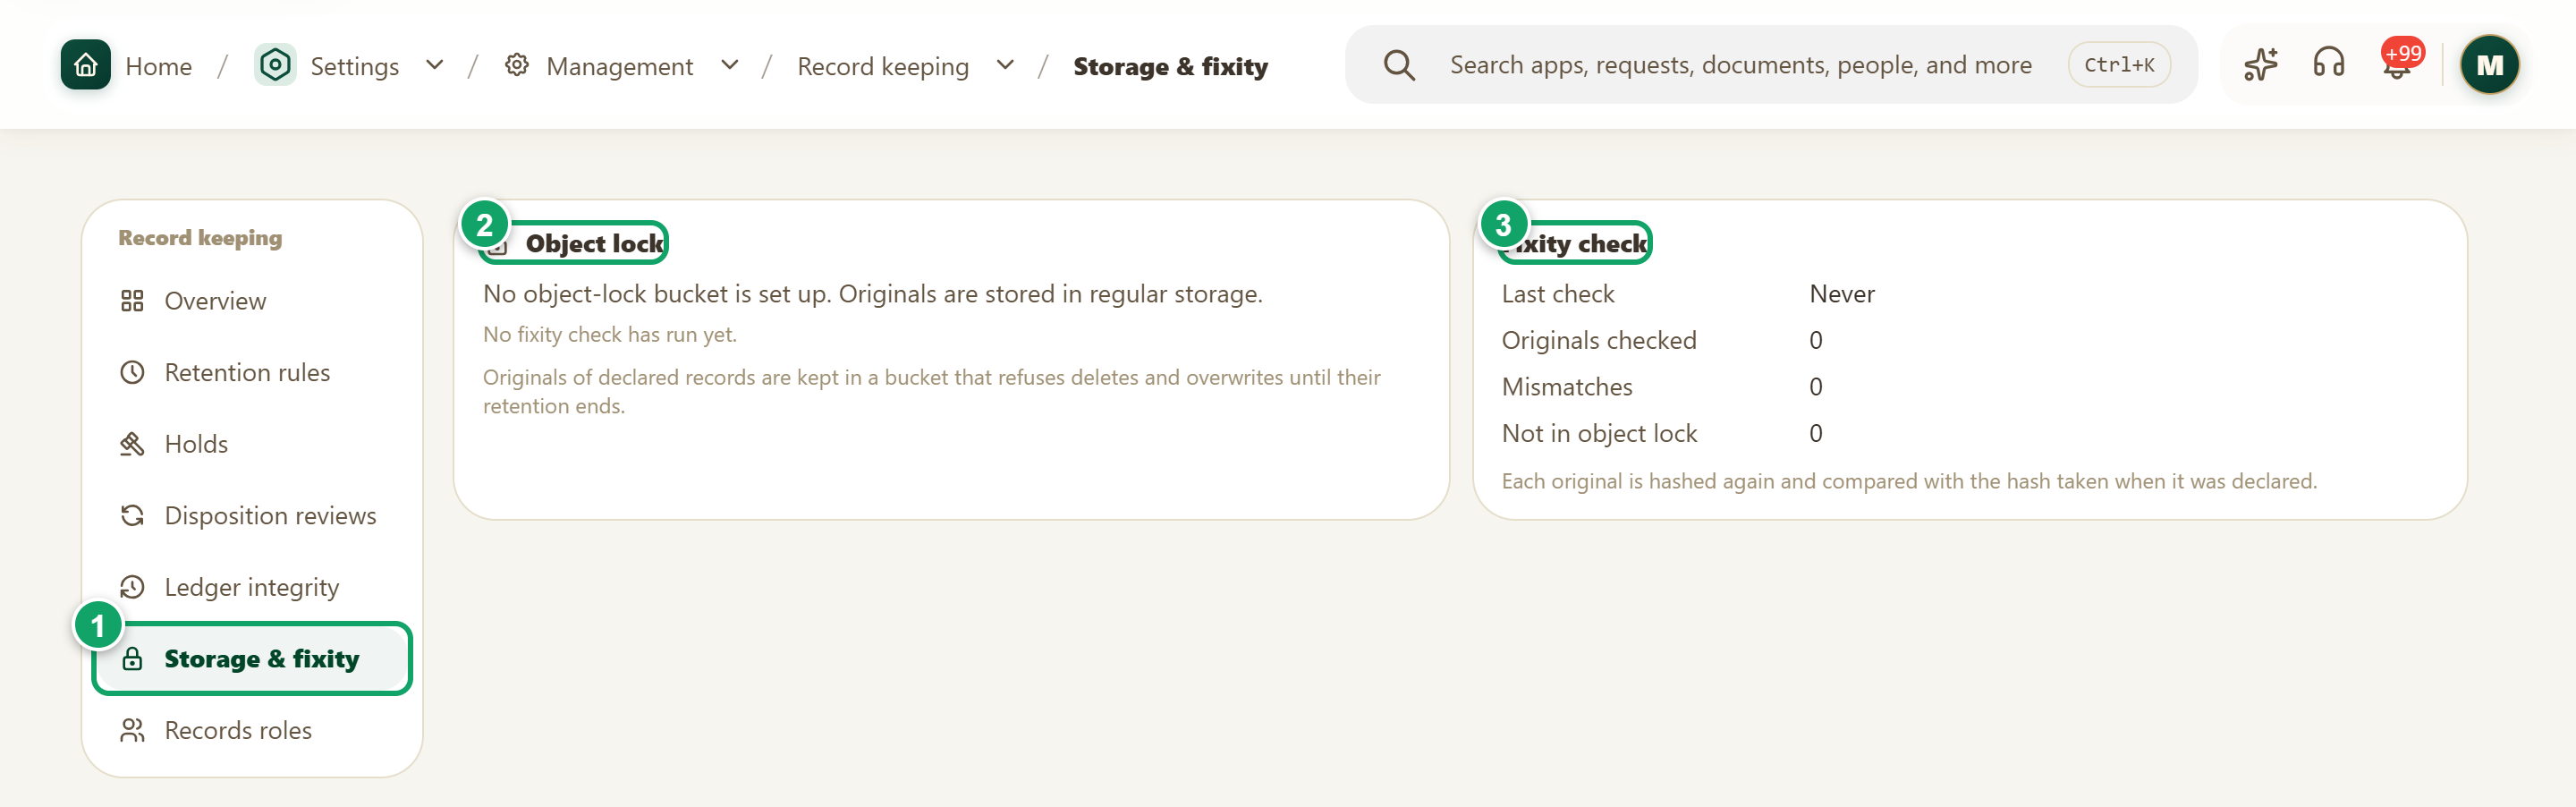
\includegraphics[width=0.95\linewidth,height=0.72\textheight,keepaspectratio]{figures/screens/ch08-record-keeping-storage-en.png}
\caption{Storage and fixity}
\label{fig:settings-record-keeping-storage-screen}
\shotnote{This page shows how the original files of declared records are protected. Here the test organization has not set this protection up, and no check has run. ① “Storage \& fixity”. ② “Object lock”: storage that refuses deletes and overwrites until the period ends. ③ “Fixity check”: compares each original’s hash with the one taken when it was declared.}
\end{figure}

\begin{figure}[H]
\centering
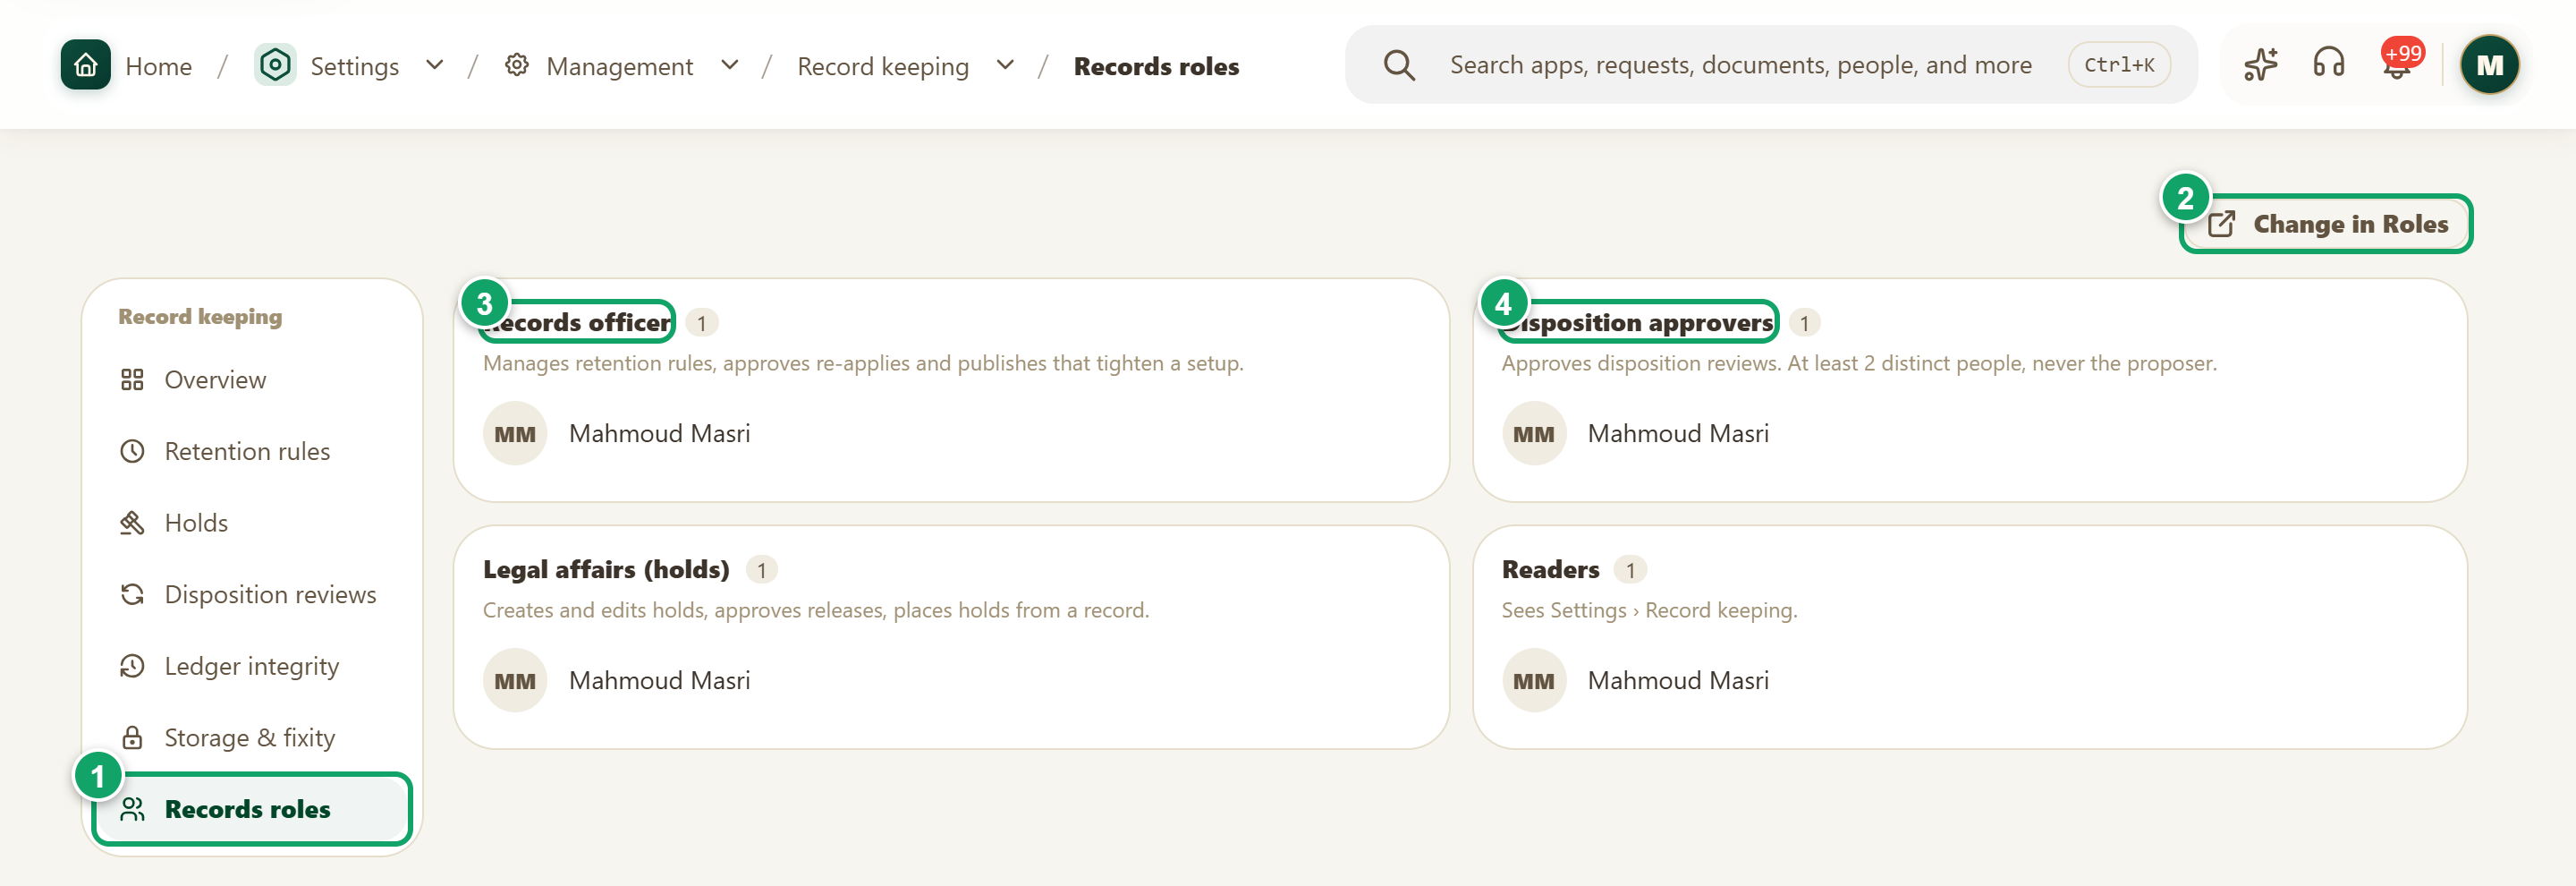
\includegraphics[width=0.95\linewidth,height=0.72\textheight,keepaspectratio]{figures/screens/ch08-record-keeping-roles-en.png}
\caption{Records roles}
\label{fig:settings-record-keeping-roles-screen}
\shotnote{This page shows who holds each responsibility but does not change it directly. Separating the roles keeps one person from both proposing and approving a disposition. ① “Records roles”. ② “Change in Roles”: takes you to the Roles page. ③ “Records officer”. ④ “Disposition approvers”.}
\end{figure}

\begin{table}[H]
\centering
\caption{What do you record in Record keeping?}
\label{tab:settings-record-keeping-fields}
\begin{tabularx}{\linewidth}{R{4.2cm} Y}
\rcHeaderRow
\thh{Section} & \thh{What you record or read}\\
“Retention rules” & Code, “Legal basis”, title, “Owner unit”, “Effective from”, “Starts at”, “Keep for” with unit and calendar, “Then”, “Approvals needed” from two to five, and “What changed”.\\
“Holds” & Type, title, “Matter”, “Review on”, reason, “Owner”, “Owner unit”, “Effect”, “Custodians” (the members whose records and files are caught) and scope.\\
“Disposition reviews” & Records, those left out, and approvals. A record can be taken out before approvals start, and the certificate is issued after the action runs.\\
“Ledger integrity” & Event count, the last signed anchor, and the record types that keep a ledger.\\
“Storage \& fixity” & Object lock status, last check, originals checked and mismatches.\\
“Records roles” & The members in “Records officer”, “Disposition approvers”, “Legal affairs (holds)” and “Readers”.\\
\end{tabularx}
\end{table}

\begin{enumerate}
\item Open “Settings”, then “Record keeping”, and start from “Overview” by reading “Needs attention”.
\item To add a rule, open “Retention rules”, press “New rule”, fill in the fields and press “Create rule”.
\item To place a hold, open “Holds”, press “New hold”, choose the type, effect and scope, then press “Create hold”.
\item To review a disposition, open the review, check its records, then press “Approve” or “Reject” if you are an approver.
\item To release a hold, open it and press “Request release”; it is released once its owner and Legal affairs agree.
\end{enumerate}

\textbf{Check:} The rule appears in the “Active” list, and the hold shows its number and caught records. A disposition review moves through its stages and runs only when approvals are complete. If your record type is missing from the overview, turn record keeping on for it in the Builder.
